\documentclass[a4paper, 12pt, twoside, openany]{mythesis}

\renewcommand{\baselinestretch}{1}       % for squeezing the draft into the page limit, do not use

% Note
% Use \textsc{Name} to separate images, videos, dataset names from the main texts.

% =============================================================================
% Commonly used packages
% =============================================================================

% For removing Package ifpdf Error
%%%%%%\let\ifpdf\relax

% For removing LaTeX Font Warning
\usepackage{lmodern}

% Add Reference in Contents
\usepackage[nottoc]{tocbibind}

% Figures
%\usepackage{subcaption}
\usepackage{float}
%\usepackage[justification=raggedright]{caption}	% makes captions ragged right - thanks to Bryce Lobdell
\usepackage{lscape} % Useful for wide tables or figures.
\usepackage{makecell}
\usepackage{sidecap}

\graphicspath{{figures}{example}}

% Algorithm
\usepackage[lined,ruled,linesnumbered]{algorithm2e}
\usepackage{algorithmic}

% Table and list
\usepackage{booktabs} % Publication quality tables
\usepackage{multirow}
\usepackage{rotating} % sideways
\newcommand{\vergap}[1]{\renewcommand{\arraystretch}{#1}}
\newcommand{\horgap}[1]{\setlength{\tabcolsep}{#1}}
%\specialrule{width}{abovespace}{belowspace}
\newcommand{\dtoprule}{\specialrule{2pt}{0pt}{2pt}}
\newcommand{\dbottomrule}{\specialrule{2pt}{0pt}{\belowrulesep}}
\usepackage{colortbl}

\usepackage{paralist}
\usepackage{enumitem}

% Math
\usepackage{bm} % Make bold, italic math symbols
\usepackage{epsfig} % for figures
\usepackage{graphicx} % another package that works for figures
\usepackage{times}
%\usepackage{mathptmx}
\usepackage{mathtools}
\usepackage{textcomp, gensymb} % math symbol
\usepackage{amssymb,amsmath,amsfonts} % Short math guide for LaTeX ftp://ftp.ams.org/pub/tex/doc/amsmath/short-math-guide.pdf
\usepackage{siunitx} % SI units
\newcommand{\norm}[1]{\left\lVert#1\right\rVert}
\newcommand{\cp}[1]{\left[#1\right]_{\times}}

% Fonts
\usepackage{units}
\usepackage{color}

% Comments
\usepackage{comment}

% Hyperlinks
\usepackage{url} % Hyphenation of URLs.
\usepackage{xcolor}
\usepackage[backref=page]{hyperref}
\hypersetup{colorlinks,breaklinks,
            urlcolor=[rgb]{0.918,0,0.545},
            linkcolor=[rgb]{0.710,0.180,0.141},
            citecolor=[rgb]{0,0.545,0.447}}
\usepackage{bookmark}
%\usepackage[pagebackref=true,breaklinks=true,colorlinks,bookmarks=false]{hyperref} % remove letterpaper=true,
%
\usepackage{slashbox}
\usepackage{xspace}
%\usepackage[table,caption=false]{xcolor}
%\usepackage{setspace}

% Better hyphenation
\usepackage{microtype}

% Appendix
\usepackage[toc,page]{appendix}

% =========================================
% Useful macros
% =========================================

% Latin abbreviations
\newcommand{\etal}{\textit{et al}.~} % ``and others'', ``and co-workers''
\newcommand{\eg}{e.g.,~} % ``for example''
\newcommand{\ie}{i.e.,~} % ``that is'', ``in other words''
\newcommand{\suchthat}{\, \mid \,}

% Math related
\DeclareMathOperator*{\argmin}{\arg\!\min}
\DeclareMathOperator*{\argmax}{\arg\!\max}
\DeclareMathOperator{\avg}{avg}
\DeclareMathOperator{\Tr}{Tr}

% Paragraph
\let\originalparagraph\paragraph
\renewcommand{\paragraph}[2][.]{\originalparagraph{#2#1}}

% Consistent margin adjustment for paragraphs, figures, and sections
\newlength\paramargin
\newlength\figmargin
\newlength\secmargin

\setlength{\secmargin}{0.0mm}
\setlength{\paramargin}{0.0mm}
\setlength{\figmargin}{0.0mm}

% References for figures, tables, equations, chapters, and sections
\newcommand{\chref}[1]{Chapter~\ref{ch:#1}}
\newcommand{\secref}[1]{Section~\ref{sec:#1}}
\newcommand{\figref}[1]{Figure~\ref{fig:#1}}
\newcommand{\tabref}[1]{Table~\ref{tab:#1}}
\newcommand{\eqnref}[1]{\eqref{eq:#1}}
\newcommand{\thmref}[1]{Theorem~\ref{#1}}
\newcommand{\prgref}[1]{Program~\ref{#1}}
\newcommand{\algref}[1]{Algorithm~\ref{#1}}
\newcommand{\clmref}[1]{Claim~\ref{#1}}
\newcommand{\lemref}[1]{Lemma~\ref{#1}}
\newcommand{\ptyref}[1]{Property~\ref{#1}}

% Comments
\long\def\ignorethis#1{}
\newcommand {\sychien}[1]{{\color{blue}\textbf{Po-Chen: }#1}\normalfont}
\newcommand {\coauthorA}[1]{{\color{red}\textbf{Co-author A: }#1}\normalfont}
\newcommand {\coauthorB}[1]{{\color{magenta}\textbf{Co-author B: }#1}\normalfont}
\newcommand {\todo}{{\textbf{\color{red}[TO-DO]\_}}}
\def\newtext#1{\textcolor{blue}{#1}}
\def\modtext#1{\textcolor{red}{#1}}

%\usepackage{ifthen}
%\ifthenelse{\equal{\final}{1}}
%{
%  \renewcommand{\sychien}[1]{}
%}
%{}

\newcommand{\tb}[1]{\textbf{#1}}
\newcommand{\mb}[1]{\mathbf{#1}}
\newcommand{\Paragraph}[1]{\noindent\textbf{#1}}

\newcommand{\jbox}[2]{
  \fbox{%
  	\begin{minipage}{#1}%
  		\hfill\vspace{#2}%
  	\end{minipage}%
  }
}

\newcommand{\jblock}[2]{%
  \begin{minipage}[t]{#1}\vspace{0cm}\centering%
  #2%
  \end{minipage}%
}
	
% Customized definition
\newcommand{\Ic}{\mathcal{I}_{c}}
\newcommand{\It}{\mathcal{I}_{t}}
\newcommand{\Ot}{\mathcal{O}_{t}}
\newcommand{\asin}{\mathrm{asin}}
\newcommand{\acos}{\mathrm{acos}}
\newcommand{\atan}{\mathrm{atan}}
\newcommand{\atanT}{\mathrm{atan2}}
\newcommand{\dotP}{\mathrm{dot}}

\usepackage{titlesec}

\renewcommand{\baselinestretch}{2}

%\hypersetup{
%    colorlinks=true,       % false: boxed links; true: colored links
%    linkcolor=blue,          % color of internal links
%    citecolor=blue,        % color of links to bibliography
%    filecolor=blue,      % color of file links
%    urlcolor=blue           % color of external links
%}

%------------------------------------
% Thesis boundary Setting
%-------------------------------------

\textwidth      = 137.0mm
\textheight     = 224.0mm
\topmargin      =  -3.0mm
\headheight     =   7.0mm
\headsep        =  10.0mm
\footskip       =   8.0mm
\oddsidemargin  =  10.6mm
\evensidemargin =  10.6mm
\hoffset = -0.2cm
%\overfullrule=5pt%%


\titleformat{\chapter}[display]   
{\normalfont\huge\bfseries}{\chaptertitlename\ \thechapter}{-20pt}{\Huge}   
\titlespacing*{\chapter}{0pt}{-60pt}{10pt}

\begin{document}

\begin{titlepage}
\pagestyle{empty}
\title{\textbf{Robot-Assisted Endodontic Treatment Based on Force-Guided Alignment and File Feedrate Control}}
\author{ \\  \\ \\
{\it Yi-Chan Li}\\
{\it Advisor: Cheng-Wei Chen} \\ \\ \\ \\ 
{\it Graduate Institute of Electronics Engineering}\\
{\it National Taiwan University} \\
{\it Taipei, Taiwan}\\ }
{\date{June 2021}}
\maketitle
\end{titlepage}


\frontmatter %turns off chapter numbering and uses roman numerals for page numbers
\chapter{Abstract}
\label{ch:abstract}
\vspace*{-10mm}
\hspace*{6mm}Advancements in robot-assisted surgery invigorates researches on robotics in the dental field. Reviewing the literature on dental robots, this thesis aims to develop a root-assisted system for endodontic treatment to improve the success rate of surgery. Considering the workspace and extreme precision in endodontic treatment, our robot-assisted system - DentiBot consists of a robot arm, an F/T sensor. System integration solutions are examined in the thesis. Moreover, to overcome the two main failures of surgery - incomplete root preparation and instrument fracture, novel ideas to perform endodontic treatment with DentiBot are presented in this thesis. First, Force-guided alignment based on admittance control is involved to calibrate the surgical path in real-time. Second, file feedrate control is addressed to protect endodontic files from fracturing. Last but not least, an algorithm based on the above functions is proposed to achieve high performance in root preparation. The technical experiments have validated the feasibility of Force-guided alignment and a pre-clinical experiment has proved file feedrate control and our proposed algorithm.




\textit{Keywords: Endodontic treatment, Robot-assisted system, Admittance control, Force-guided alignment, File feedrate control, Instrument fracture}

 




\tableofcontents
\listoffigures
\listoftables

%------------------------------------
% Thesis Body -- begin
%------------------------------------

\titlespacing*{\chapter}{0pt}{-40pt}{35pt}

\mainmatter %turns on chapter numbering, resets page numbering and uses arabic numerals for page numbers

\chapter{Introduction}
Endodontic treatment, also known as root canal treatment and nerve extraction, is performed to cure an infected tooth. The procedure of endodontic treatment is divided into three parts - Opening, Cleaning, and Filling shown in  Figure \ref{fig:endo-procedure}.
\begin{figure}[htbp]
\begin{center}
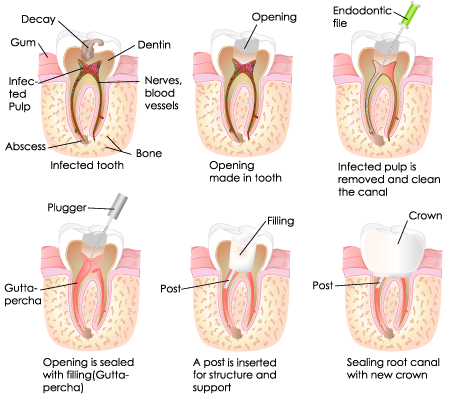
\includegraphics[width=0.8\linewidth]{Images/endo-procedure.png}
\end{center}
\caption{
The endodontic therapy steps
}\label{fig:endo-procedure}
\end{figure}
\newpage
An infected tooth results from periodontal disease, attrition, trauma, or decay. Once the dental pulp is infected, it causes an irreversible inflammation and let patients confront a root canal treatment. Figure \ref{fig:endo-procedure} shows an infected tooth and its dental pulp, which is composed of blood vessels, nerves, connective tissues, and lymphatics. In the "Opening" step, an experienced dentist drills the crown of infected tooth to remove the dentin and expose the infected pulp inside the canal to the air. Next, in the "Cleaning" step the dentist uses an endodontic file which is a flexible reamer to remove the infected pulp. Then, in the "Filling" step the dentist uses a dental plugger to fill the empty root canal with Gutta-percha which is a plastic substance. "Filling" can prevent cross infection between root canals because the cured teeth remains many invisible and inaccessible pulp tissue. Finally the dentist seals root canal with new crown to protect cured root canal. 
\par
"Cleaning" is of paramount importance in a whole treatment because untreated cleaning will result in pulp necrosis, apical abscess, periodontal ligament inflammation, or even cellulitis. If there are many remained infected pulp after root canal treatment, the surgery should be operated on again.
\section{Motivation}
The performance of the endodontic treatment depends on the dentist's own long-term experience. A qualified dentist can operate the endodontic treatment and accumulate their experience to increase the success rate. With many experiences, dentists can acquire an endodontist license. According to statistics from the Ministry of Health and Welfare, R.O.C. (Taiwan), the number of dentists in Taiwan is $15,178$. However, according to The Academy of Endodontology, R.O.C. (Taiwan), there are only $238$ dentists to acquire an endodontist license due to the expertise of endodontics. Besides, Root canal treatment is tedious and time-consuming due to complicated conditions of each tooth, a patient who suffered from an infected tooth spends much time see a dentist It takes at least two to three rounds, even spends more than two months in the worst case. 
\par
Therefore, our team looks forward to designing a robot-assisted system to help a dentist finish the root canal treatment. With the system, we wish it can increase the success rate for dentists and provide patients a safe surgery.

\section{Previous Work and Problem Definition}
(Previous work: briefly mention the existing dental robots)
\par\noindent
(Problem definition:
1.	Assist dentists to operate RCT and focus on cleaning procedure
2.	Root canal cannot be visually observed and is too small to clean well
3.	Risk of file breakage)		
\par\noindent
Instruments fracture and perforation are two problems that commonly occur during the therapy. Removal of broken files is both technically difficult and therefore it is important to reduce the probability of fracture. In addition, root canal treatment also requires repeatedly drilling in order to clean the canal thoroughly.  This repetitive action of root canal treatment is tedious and time-consuming. Therefore, we designed an automatic endodontic robot to improve the time-efficiency and to reduce the occurrence of instrument fracture in endodontic surgery.
The root canal cleaning is a big challenge in and of itself
There is one robotic system that is designed to perform endodontic therapy. In Intelligent Micro Robot Development for Minimum Invasive Endodontic Treatment [3] , they proposed a micro robot performing root canal treatment with the assistance of 3D computer model system. It is designed to accomplish endodontic therapy with path planned according to the 3D model. However, the problem of instruments fracture still remains. 
In this paper, a torque monitoring method is proposed. The main causes of fractured files are torsional fracture and flexural fatigue, account for 55.7\% and 44.3\% separately [5]. Therefore, we use current feedback to keep track of the torque which the file is bearing during the endodontic treatment. This torque monitoring system is implemented on an endodontic robot prototype we built. We primarily focus on the cleaning and shaping step since it’s the key step to a successful root canal treatment. With the robot prototype and torque monitoring system, the possibility of instrument fracture can be reduced. Besides, the repetitive action during the drilling step can be performed by the robot.			
\section{The Proposed Method}
(Solutions: (be consistent with problem definition)
1.	Build a robot-assisted system and enable it to drill
2.	Force-guided alignment 
3.	Control the file rotation speed
B.	Prospect:
\par\noindent
(Prospect: Move to the infected teeth$\longrightarrow $Root canal searching$\longrightarrow $Repetitive drilling$\longrightarrow $Apex Detection)						
\section{Main Contributions of the Thesis}
\begin{enumerate}
	\item	Integrate a 6-DoF robotic manipulator with 6-DoF F/T sensor for performing endodontic treatment.
	\item	Develop a framework for robot alignment regarding the position and orientation of root canal. 
	\item	Protect the endodontic file from fracturing by controlling file rotation speed.
\end{enumerate}
\section{Organization of the Thesis}
\chapter{State-of-the-Art}
\hspace*{6mm}
To comprehensively contemplate requirements of an endodontic robot such as workspace, payload, clinical problems, technical and clinical literatures are involved. Recent literatures have revealed that researchers have seen the use of dental robot for implant surgery \cite{Kim2009ASO}\cite{Li2019ACD}\cite{9026216}. There was a domestic team dedicating to develop an endodontic robot \cite{dong2006wip}. Endodontic file has its physical property
\section{Dental Robot}
\hspace*{6mm}There is a commercial robot, YOMI  \cite{bolding2021accuracy}. YOMI has received the clearance from FDA and has performed more than $2,700$ times surgery in the USA. In the pandemic of Covid-19 in 2020, YOMI provided non-contact surgery between dentists and patients due to its automatic robotic system. 
\begin{figure}[htbp]
\begin{center}
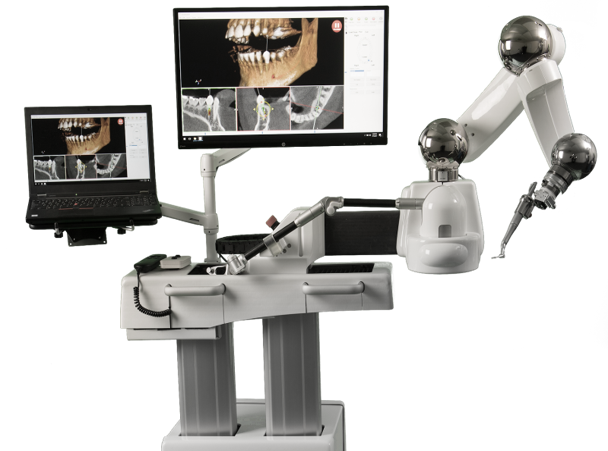
\includegraphics[width=0.9\linewidth]{Images/YOMI.png}
\caption{
YOMI
}\label{fig:YOMI}
\end{center}
\end{figure}
There is one robotic system that is designed to perform the endodontic therapy. In Intelligent Micro Robot Development for Minimum Invasive Endodontic Treatment \cite{dong2010design}, they proposed a micro robot performing root canal treatment with the assistance
of 3D computer model system. It utilizes the 3D model to plan the corresponding path to accomplish an endodontic treatment.

There are more and more robots which applied to specific surgery. In the dental field, the majority of robotic applications are in implant surgery. The researchers in Chosun University built a dental implant robot \cite{Kim2009ASO}, a remote center of motion (RCM) mechanism. Li, J. et al. designed a robotic system using a soft bracing technique to drill teeth \cite{Li2019ACD}. Also, there is the first commercial implant robot, YOMI, developed by Neosis \cite{web3}. However, there was one and only one robot for the endodontic treatment. The domestic researcher Janet Dong and his team proposed a microrobot performing root canal treatment with the assistance of a 3D computer model system. However, the study using 3D model belongs to pre-operation.
\begin{figure}[htbp]
\begin{center}
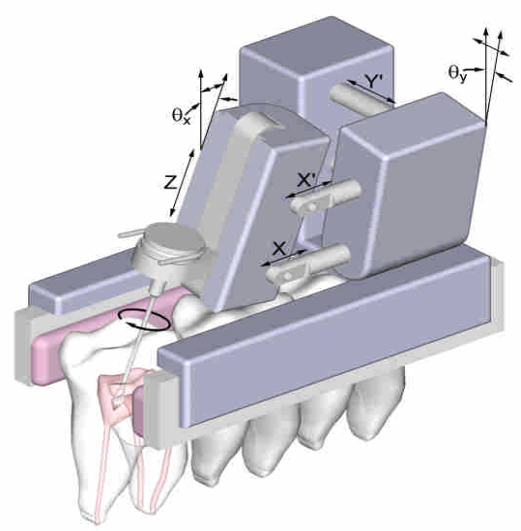
\includegraphics[width=0.7\linewidth]{Images/NCTU_1.png}
\caption{
Multi-purpose micro-machine for automatic endodontic treatment
}\label{fig:NCTU_1}
\end{center}
\end{figure}
\section{Peg-in-Hole}
\section{Torque Control}
A.	YOMI – commercial robot
B.	HK - dental implant robot
C.	Korean - dental implant robot
D.	NCTU – RCT robot

\section{File property}
\hspace*{6mm}To protect the endodontic file from fracturing, we need to be familiar with its physical property and its correct operations. We delve into the physical properties of an endodontic file. A file is made of alloys of Nickel and Titanium, which is a superelastic material. The Ni-Ti file has significantly more elastic and incorruptible properties. This feature allows it to bend when inserted into a curve root canal and thereby reduces the possibility of stuck.
\begin{figure}[htbp]
\begin{center}
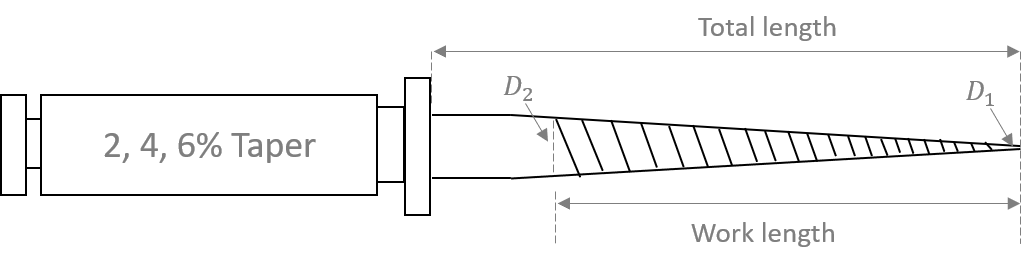
\includegraphics[width=1\linewidth]{Images/Endodontic_File.png}
\caption{The illustration of an endodontic file
}\label{fig: Endodontic File}
\end{center}
\end{figure}	
\par
In Fig \ref{fig: Endodontic File}, an endodontic file is illustrated. There are four types of total length - $21$, $25$, $28$, and $31$ mm. They all have the same work length - $16$ mm. Each file has their own number such as $\#15, \#20, \#25, \cdots, \#40$, which represent the diameter of files. Take a $\#15$ file with $2\%$ taper for example,
\par\noindent
the diameter of the tooltip $D_1$ is
\begin{equation*}
\begin{split}
15/100=0.15 \text{ (mm)}
\end{split}
\end{equation*}
and the diameter at the end of the work length $D_2$ is
\begin{equation*}
\begin{split}
0.15 + 16 \cdot 6\% = 1.11 \text{ (mm)}
\end{split}
\end{equation*}
						
\chapter{Design and Analysis of the Dental Surgical Robot - DentiBot}
\section{Requirement and Specification}
(Payload, resolution and workspace)														\par\noindent
(Why not RCM mechanism)		
															
\section{Design of the DentiBot}
As discussed in previous section, we have to select suitable devices according to those requirements. First, We choose Meca500 manufactured by Mecadamic Inc. as our 6 DOF robot arm. Its feature is high repeatability (precision: 5 $\mu m$) and it is equipped with zero-backlash speed reducers. In addition, it is compact and portable for laboratory investigation. Second, Mini40 manufactured by ATI Inc. is the corresponding F/T sensor with three force and three torque detections. As for the end effector, we modify a existing dental handpiece which equips a tool change mechanism. The modified handpiece weights around 139 grams. We also design  adapters so as to assemble these devices.
\par\noindent
DentiBot has seven degree of freedom. 6 DOF is come from Meca500, and the other DOF is owing to our modified handpiece. The rotation of root canal file is driven by a servo motor whose maximum rotation speed is more than 600 rpm.																		
\section{Kinematics Analysis}
\label{sec:kinematics}
The purpose of this section and section \ref{sec:ref_robot} is to serve as a tutorial and provide some important approaches when combining a robot arm and an end effector. We derive the forward and inverse kinematics in section \ref{sec:forward} and describe Jacobian matrix in section \ref{sec:jacobian}. 

\subsection{Coordinate Definition}
In Fig \ref{fig:frames} , we define frame\{0\} to frame\{6\} which represent each frame of axis of the Meca500, frame\{S\} which represent the frame of the ATI-mini40 and frame\{H\} which represent the frame of the handpiece.
\begin{figure}[htbp]
\begin{center}
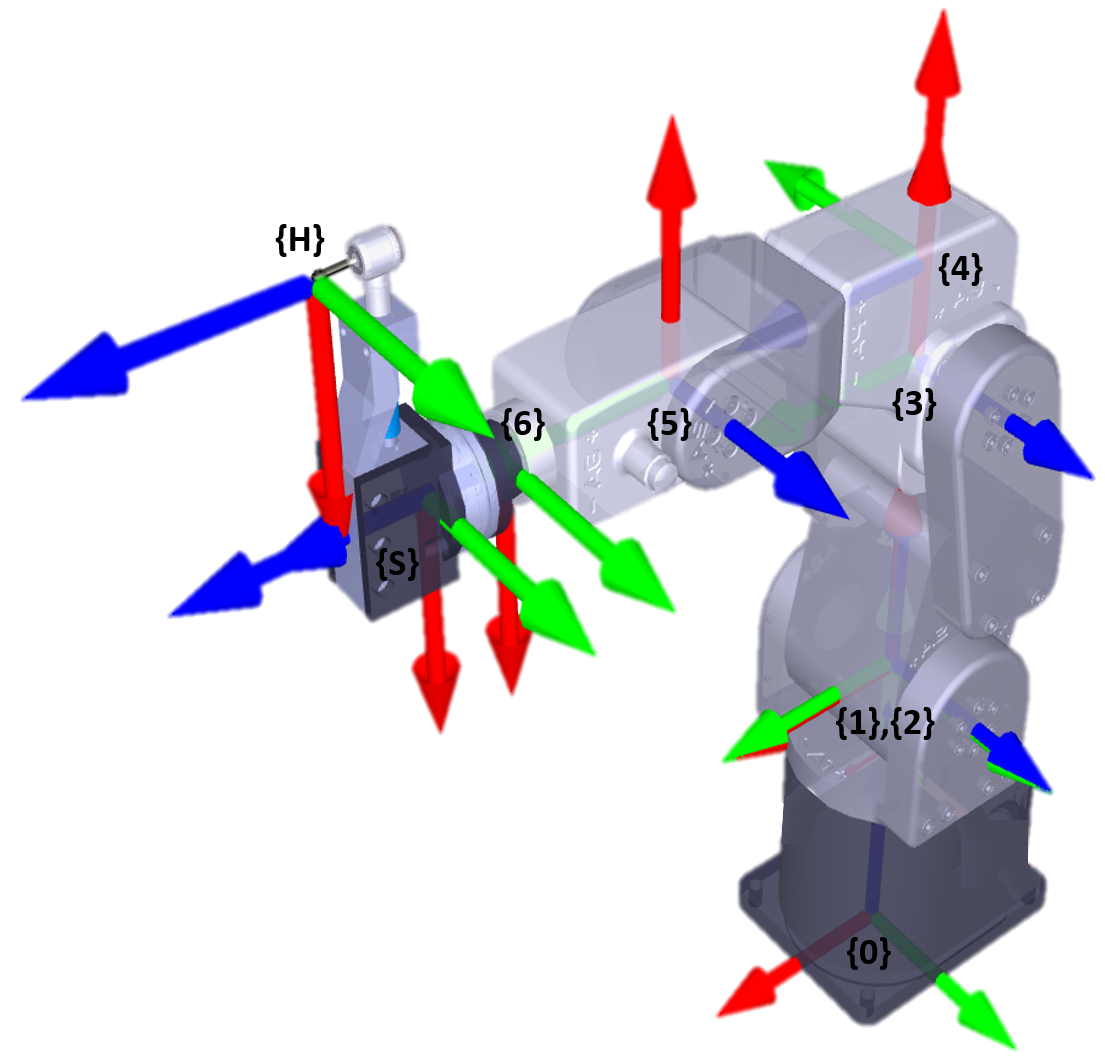
\includegraphics[width=0.72\linewidth]{Images/Coordinates.png}
\caption{
Coordinate Definition
}\label{fig:frames}
\end{center}
\end{figure} 
\subsection{Forward and Inverse Kinematics}
\label{sec:forward}
\begin{table}[htbp]
\centering
\caption{Denavit-Hartenberg parameters of Meca500}
\label{tab:DHtable}
\begin{tabular}{ccccc} 
\hline \hline
$i$ (link number)		&$\alpha _{i-1}$ (deg)	&$a_{i-1}$ (mm)	& $\theta _i$ (deg)			&$d_i$ (mm)	\\
\hline
1   					&0    					&0				&$\theta _1$				&135 \\
2   					&-90   					&0				&$\theta _2$				&0 \\
3  						&0    					&135			&$\theta _3$ 				&0 \\
4   					&-90    				&38				&$\theta _4$ 				&120 \\
5   					&90   					&0				&$\theta _5$ 				&0 \\
6						&-90  					&0				&$\theta _6$ 				&70 \\
\hline\hline
\end{tabular}
\end{table}
Denavit-Hartenberg parameters are shown as Table \ref{tab:DHtable}. Then, the forward kinematics of Meca500 is derived as
\begin{equation}
\begin{split}
^0_6\mathbf{T} =
\ ^0_1\mathbf{T} \cdot \ ^1_2\mathbf{T} \cdot \ ^2_3\mathbf{T} \cdot \ ^3_4\mathbf{T} \cdot \ ^4_5\mathbf{T} \cdot \ ^5_6\mathbf{T} =
\begin{bmatrix}
^0_6\mathbf{R}	&^0\boldsymbol{p}_\mathrm{6org}\\
0				&1\\
\end{bmatrix}\\
\end{split}
\end{equation}\label{eq:translation matrix}
where $^0_6\mathbf{R}$ is the rotation matrix from frame\{6\} to frame\{0\}, $^0\boldsymbol{p}_\mathrm{6org}$ is the origin of the frame\{6\} observed from frame\{0\}. All detailed indexes of $^0_6\mathbf{T}$ are shown as Appendix \ref{appendix:forward}
\par
Incidentally, there is an alternative to calculate the transformation matrix of Meca500. We can use command "GetPose" to obtain (x,y,z,$\alpha$,$\beta$,$\gamma$). Then, we can use this information to derive the following equation.
\begin{equation}
\begin{split}
^0_6\mathbf{T} 
&= 
\begin{bmatrix}
\mathbf{R_x(\alpha ) \cdot R_y(\beta ) \cdot R_z(\gamma )} 
& \begin{matrix}
x\\ 
y\\ 
z
\end{matrix}\\ 
0 & 1
\end{bmatrix}\\
&= 
\begin{bmatrix} 
c_\beta c_\gamma 										& -c_\beta s_\gamma 									& s_\beta 					&x\\ 
c_\alpha s_\gamma +  s_\alpha s_\beta c_\gamma 			& c_\alpha c_\gamma -  s_\alpha s_\beta s_\gamma		& -s_\alpha c_\beta			&y\\ 
s_\alpha s_\gamma -  c_\alpha s_\beta c_\gamma 			& s_\alpha c_\gamma +  c_\alpha s_\beta s_\gamma 		& c_\alpha c_\beta 			&z\\ 
0 														&0 														&0							&1
\end{bmatrix}
\end{split}
\end{equation}
where $C_{\star} $, $ S_{\star}$ denote $\cos \left(\star \right)$, $\sin \left(\star \right)$; $\alpha ,\beta ,\gamma$ are in representation of Euler angle.
\subsection{Jacobian matrix} 
\label{sec:jacobian}
Here we evaluate geometric Jacobian based on frame\{0\}, geometric Jacobian based on frame\{6\} and analytical Jacobian.
\par
First and foremost, we should clarify the difference between geometric Jacobian and analytical Jacobian. They both use the same linear velocity but consider different angular velocity. The angular velocity which geometric Jacobian applies is relevant to the axis angles ($\theta _x$,$\theta _y$,$\theta _z$). In contrast, the angular velocity analytical which Jacobian contemplates is related to the orientation ($\alpha$,$\beta$,$\gamma$) of the end effector.
\subsubsection{Geometric Jacobian Based on Frame\{0\}}
Before proceeding to examine the geometric Jacobian matrix, it will be necessary to find the relationship between the position and joints' angles and the relationship between the axis angle and the joints' angles.
\par\noindent
On the basis of the translation matrix in Equation \ref{eq:translation matrix}, we obtain the relationship between the position and joints' angles.
\begin{equation}
\begin{split}
^0\boldsymbol{p}_\mathrm{6org}
= 
\begin{bmatrix}
x\\
y\\
z\\
\end{bmatrix} 
=
\begin{bmatrix}
x(\theta _1, \theta _2, \cdots, \theta _6)\\
y(\theta _1, \theta _2, \cdots, \theta _6)\\
z(\theta _1, \theta _2, \cdots, \theta _6)
\end{bmatrix} 
\end{split}
\end{equation}\label{eq:lin vel}
Moreover, we dissect the relationship between the axis angle and joints' angles.
\begin{equation}
\begin{split}
\begin{bmatrix}
\theta _x \\
\theta _y \\
\theta _z 
\end{bmatrix}
=
\ ^0_1\mathbf{R}
\begin{bmatrix}
0 \\ 
0 \\ 
\theta _1
\end{bmatrix}
+
\ ^0_2\mathbf{R}
\begin{bmatrix}
0 \\ 
0 \\ 
\theta _2
\end{bmatrix}
+
\ ^0_3\mathbf{R}
\begin{bmatrix}
0 \\ 
0 \\ 
\theta _3
\end{bmatrix}
+
\ ^0_4\mathbf{R}
\begin{bmatrix}
0 \\ 
0 \\ 
\theta _4
\end{bmatrix}
+
\ ^0_5\mathbf{R}
\begin{bmatrix}
0 \\ 
0 \\ 
\theta _5
\end{bmatrix}
+
\ ^0_6\mathbf{R}
\begin{bmatrix}
0 \\ 
0 \\ 
\theta _6
\end{bmatrix}
\end{split}
\end{equation}\label{eq:ang vel_axis}
We can differentiate Equation \ref{eq:lin vel} and \ref{eq:ang vel_axis} to obtain Jacobian matrices.
\begin{equation}
\begin{split}
\boldsymbol{v} 
= 
\begin{bmatrix}
\dot{x}\\
\dot{y}\\
\dot{z}
\end{bmatrix}
=
\mathbf{J_{gv}} \cdot \boldsymbol{\dot{q}}
,\ 
\boldsymbol{w} 
= 
\begin{bmatrix}
\dot{\theta _x}\\
\dot{\theta _y}\\
\dot{\theta _z}
\end{bmatrix}
=
\mathbf{J_{gw}} \cdot \boldsymbol{\dot{q}}
\end{split}
\end{equation}
where
\begin{equation*}
\begin{split}
\mathbf{J_{gv}} =
\begin{bmatrix}
\frac{\partial x}{\partial \theta _1}	&\frac{\partial x}{\partial \theta _2}	&\cdots		&\frac{\partial x}{\partial \theta _6}\\
\frac{\partial y}{\partial \theta _1}	&\frac{\partial y}{\partial \theta _2}	&\cdots		&\frac{\partial y}{\partial \theta _6}\\
\frac{\partial z}{\partial \theta _1}	&\frac{\partial z}{\partial \theta _2}	&\cdots		&\frac{\partial z}{\partial \theta _6}
\end{bmatrix}
,\ \mathbf{J_{gw}} = 
\begin{bmatrix}
\frac{\partial \theta _x}{\partial \theta _1}	&\frac{\partial \theta _x}{\partial \theta _2}	&\cdots		&\frac{\partial \theta _x}{\partial \theta _6}\\
\frac{\partial \theta _y}{\partial \theta _1}	&\frac{\partial \theta _y}{\partial \theta _2}	&\cdots		&\frac{\partial \theta _y}{\partial \theta _6}\\
\frac{\partial \theta _z}{\partial \theta _1}	&\frac{\partial \theta _z}{\partial \theta _2}	&\cdots		&\frac{\partial \theta _z}{\partial \theta _6}
\end{bmatrix} 
,\ \boldsymbol{\dot{q}}
=
\begin{bmatrix}
\dot{\theta _1} \\ 
\dot{\theta _2} \\ 
\dot{\theta _3} \\ 
\dot{\theta _4} \\ 
\dot{\theta _5} \\ 
\dot{\theta _6} 
\end{bmatrix}\\
\end{split}
\end{equation*}
As a result, the geometric Jacobian matrix based on frame{0} $\mathbf{^0J_g}$ is derived as
\begin{equation}
\label{eq:jg0}
\begin{split}
\boldsymbol{\dot{x}} = \ \mathbf{^0\!J_g} \cdot \boldsymbol{\dot{q}}
,\ \ 
\boldsymbol{\dot{q}} = \ \mathbf{^0\!J_g^{-1}} \cdot \boldsymbol{\dot{x}}
\end{split}
\end{equation}
where
\begin{equation}
\begin{split}
\boldsymbol{\dot{x}}
=
\begin{bmatrix}
\dot{x}\\
\dot{y}\\
\dot{z}\\
\dot{\theta _x}\\
\dot{\theta _y}\\
\dot{\theta _z}
\end{bmatrix}_{\!\{0\}}
,\ 
\boldsymbol{\dot{q}}
=
\begin{bmatrix}
\dot{\theta _1} \\ 
\dot{\theta _2} \\ 
\dot{\theta _3} \\ 
\dot{\theta _4} \\ 
\dot{\theta _5} \\ 
\dot{\theta _6} 
\end{bmatrix}
\end{split}
\end{equation}
There is a further derivation. In terms of the Jacobian matrix, we can derive the other property.
\begin{equation}
\begin{split}
\boldsymbol{\tau } = \mathbf{^0\!J^\top _g} \cdot \boldsymbol{f}\ \ \ \ 
\Leftrightarrow \ \ \ \ 
\begin{bmatrix}
\tau_{\theta _1} \\ 
\tau_{\theta _2} \\ 
\tau_{\theta _3} \\ 
\tau_{\theta _4} \\ 
\tau_{\theta _5} \\ 
\tau_{\theta _6} \\ 
\end{bmatrix}
=
\mathbf{^0\!J^\top _g} 
\cdot
\begin{bmatrix}
f_x \\ 
f_y \\ 
f_z \\ 
\tau_{x} \\ 
\tau_{y} \\ 
\tau_{z}
\end{bmatrix}
\end{split}
\end{equation}
where $\boldsymbol{\tau }$ is the vector of joints' torques and $\boldsymbol{f}$ is the vector composed of inertial forces and torques of the robot arm.
\subsubsection{Geometric Jacobian Based on Frame\{6\}}
\label{sec:jg6}
Why we need geometric Jacobian based on frame\{6\} is that in section \ref{sec:adm ctrl} we will apply admittance control and it will use F/T sensor mounted on frame\{6\} instead of frame\{0\} to detect forces and torques. To start with Equation \ref{eq:jg0}
\begin{equation}
\begin{split}
\begin{bmatrix}
\dot{x}\\
\dot{y}\\
\dot{z}\\
\dot{\theta _x}\\
\dot{\theta _y}\\
\dot{\theta _z}
\end{bmatrix}_{\!\{0\}}
=
\mathbf{^0\!J_g} \cdot 
\begin{bmatrix}
\dot{\theta _1} \\ 
\dot{\theta _2} \\ 
\dot{\theta _3} \\ 
\dot{\theta _4} \\ 
\dot{\theta _5} \\ 
\dot{\theta _6} 
\end{bmatrix}\\
\end{split}
\end{equation}
Then, left-multiply a matrix. 
\begin{equation}
\label{eq:jg6_leftmul}
\begin{split}
\begin{bmatrix}
^0_6\mathbf{R} & 0_{ 3\times 3} \\ 
0_{ 3\times 3} & ^0_6\mathbf{R}
\end{bmatrix}
\begin{bmatrix}
\dot{x}\\
\dot{y}\\
\dot{z}\\
\dot{\theta _x}\\
\dot{\theta _y}\\
\dot{\theta _z}
\end{bmatrix}_{\!\{0\}}
=
\begin{bmatrix}
^0_6\mathbf{R} & 0_{ 3\times 3} \\ 
0_{ 3\times 3} & ^0_6\mathbf{R}
\end{bmatrix}
\mathbf{^0\!J_g} \cdot 
\begin{bmatrix}
\dot{\theta _1} \\ 
\dot{\theta _2} \\ 
\dot{\theta _3} \\ 
\dot{\theta _4} \\ 
\dot{\theta _5} \\ 
\dot{\theta _6} 
\end{bmatrix}\\
\end{split}
\end{equation}
According to the transformation coordinate relationship between frame\{0\} and frame\{6\},
\begin{equation}
\begin{split}
\begin{bmatrix}
\dot{x}\\ 
\dot{y}\\ 
\dot{z}\\ 
\dot{\theta_x}\\ 
\dot{\theta_y}\\
\dot{\theta_z} 
\end{bmatrix}_{\!\{6\}}
=
\begin{bmatrix}
^0_6\mathbf{R} & 0_{ 3\times 3} \\ 
0_{ 3\times 3} & ^0_6\mathbf{R}
\end{bmatrix}
\begin{bmatrix}
\dot{x}\\ 
\dot{y}\\ 
\dot{z}\\ 
\dot{\theta_x}\\ 
\dot{\theta_y}\\
\dot{\theta_z} 
\end{bmatrix}_{\!\{0\}}
\end{split}
\end{equation}
substitute it into Eq \ref{eq:jg6_leftmul}, we can observe a essential equation.
\begin{equation}
\begin{split}
\mathbf{^6\!J_g}
= 
\begin{bmatrix}
^0_6\mathbf{R} & 0_{ 3\times 3} \\ 
0_{ 3\times 3} & ^0_6\mathbf{R}
\end{bmatrix}
\cdot
\mathbf{^0\!J_g}
\end{split}
\end{equation}
Notably,
\begin{equation}
\label{eq:jg6}
\begin{split}
\boldsymbol{\dot{x}} = \ \mathbf{^6\!J_g} \cdot \boldsymbol{\dot{q}}
,\ \ 
\boldsymbol{\dot{q}} = \ \mathbf{^6\!J_g^{-1}} \cdot \boldsymbol{\dot{x}}
\end{split}
\end{equation}
where
\begin{equation*}
\begin{split}
\boldsymbol{\dot{x}}
=
\begin{bmatrix}
\dot{x}\\
\dot{y}\\
\dot{z}\\
\dot{\theta _x}\\
\dot{\theta _y}\\
\dot{\theta _z}
\end{bmatrix}_{\!\{6\}}
,\ 
\boldsymbol{\dot{q}}
=
\begin{bmatrix}
\dot{\theta _1} \\ 
\dot{\theta _2} \\ 
\dot{\theta _3} \\ 
\dot{\theta _4} \\ 
\dot{\theta _5} \\ 
\dot{\theta _6} 
\end{bmatrix}
\end{split}
\end{equation*}
\subsubsection{Analytical Jacobian}
The linear velocity of analytical Jacobian and of geometric Jacobian is the same as shown in Eq \ref{eq:lin vel}. Nevertheless, as for angular velocity, analytical Jacobian takes the the orientation ($\alpha$,$\beta$,$\gamma$) of the end effector into consideration. First of all, we investigate the relationship between the axis angle and the orientation of the end effector as following.
\begin{equation}
\begin{split}
\begin{bmatrix}
\theta _x \\ 
\theta _y \\ 
\theta _z
\end{bmatrix}
&=
\begin{bmatrix}
\alpha \\ 
0\\ 
0
\end{bmatrix}
+
R_x(\alpha)
\begin{bmatrix}
0 \\ 
\beta \\ 
0
\end{bmatrix}
+
R_x(\alpha)R_y(\beta)
\begin{bmatrix}
0 \\ 
0\\ 
\gamma
\end{bmatrix}\\
&=
\begin{bmatrix}
1 & 0 & S_\beta \\ 
0 & C_\alpha & -S_\alpha C_\beta \\ 
0 & S_\alpha & C_\alpha C_\beta
\end{bmatrix}
\begin{bmatrix}
\alpha \\ 
\beta\\ 
\gamma
\end{bmatrix}
\end{split}
\end{equation}
Then, utilize this generalized vector to get its Jacobian matrix $\mathbf{J_{we}}$.
\begin{equation}
\begin{split}
\begin{bmatrix}
\dot{\theta _x} \\ 
\dot{\theta _y} \\ 
\dot{\theta _z}
\end{bmatrix}
=
\mathbf{J_{\!we}}
\cdot
\begin{bmatrix}
\dot{\alpha} \\ 
\dot{\beta} \\ 
\dot{\gamma}
\end{bmatrix}
\end{split}
\end{equation}
where
\begin{equation}
\begin{split}
\mathbf{J_{we}}
=
\begin{bmatrix}
1														& \gamma C_{\beta}							& S_{\beta}\\
- \beta S_{\alpha} -  \gamma C_{\alpha}C_{\beta}		& C_{\alpha} +  \gamma S_{\alpha}S_{\beta}	& -C_{\beta}S_{\alpha}\\
\beta C_{\alpha} -  \gamma C_{\beta}S_{\alpha}			& S_{\alpha} -  \gamma C_{\alpha}S_{\beta}	&  C_{\alpha}C_{\beta}
\end{bmatrix}
\end{split}
\end{equation}
Therefore,
\begin{equation}
\begin{split}
\begin{bmatrix}
\dot{x} \\
\dot{y} \\
\dot{z} \\
\dot{\theta _x} \\
\dot{\theta _y} \\
\dot{\theta _z} 
\end{bmatrix}
=
\begin{bmatrix}
\mathbf{I}_{3\times 3} & 0_{3\times 3}\\
0_{3\times 3} & \mathbf{J_{we}}
\end{bmatrix}
\begin{bmatrix}
\dot{x} \\
\dot{y} \\
\dot{z} \\
\dot{\alpha} \\ 
\dot{\beta} \\ 
\dot{\gamma} 
\end{bmatrix}
\end{split}
\end{equation}
Finally, we obtain the relationship between geometric and analytical Jacobian.
\begin{equation}
\begin{split}
\mathbf{J_g} = 
\begin{bmatrix}
\mathbf{I}_{3\times 3} & 0_{3\times 3}\\
0_{3\times 3} & \mathbf{J_{we}}
\end{bmatrix}
\mathbf{J_a},\ 
\mathbf{J_g} = 
\begin{bmatrix}
\mathbf{I}_{3\times 3} & 0_{3\times 3}\\
0_{3\times 3} & \mathbf{J_{we}^{-1}}
\end{bmatrix}
\mathbf{J_a}
\end{split}
\end{equation}

\section{Coordinate Transformation of the Robot Arm}
\label{sec:ref_robot}
So far, with forward and inverse kinematics the robot arm can translate and rotate around frame\{6\}. However the origin of the frame\{6\} is not considered to be an operating point. Because the F/T sensor and a detachable end effector will be both mounted on the wrist, the position of the tool tip is exactly what we want. That means we should let the robot arm know how to translate and rotate in frame\{T\} instead of frame\{6\}. If we have translation and rotation information of the tool tip, there is an easy way to directly give these above information to the robot arm. SetTRF (x,y,z,$\alpha$,$\beta$,$\gamma$) is the command of the robot arm, whose (x,y,z) is translation vector and ($\alpha$,$\beta$,$\gamma$) is rotation vector in representation of Euler angle .
\par
For the purpose of obtaining translation and rotation vector, we respectively introduce Tool Center Point in section \ref{sec:tcp} to find the translation vector and propose an approach in section \ref{sec:rot inf} to find the rotation vector.							
\subsection{Translation Analysis - Tool Center Point}
\label{sec:tcp}
\begin{figure}[htbp]
\begin{center}
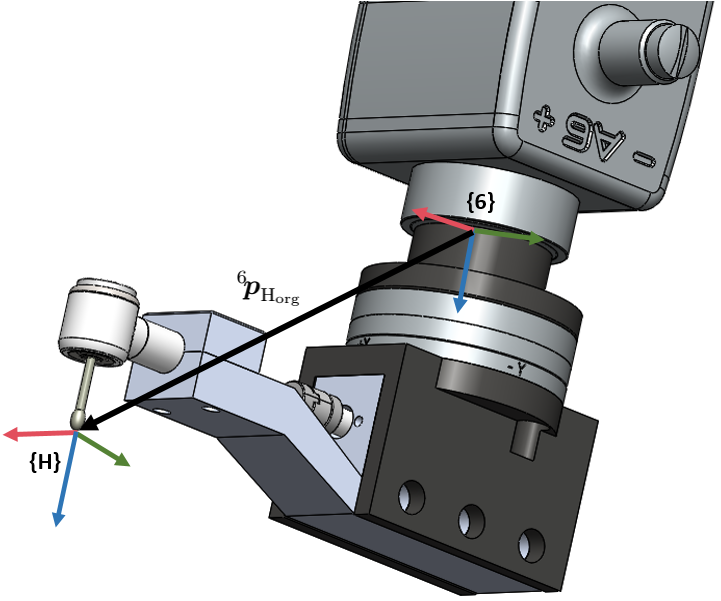
\includegraphics[width=0.7\linewidth]{Images/TCP.png}
\caption{
Schematic diagram for Tool Center Point. The translation vector $^\mathrm{6}\!\boldsymbol{p}_\mathrm{H_{org}}$ denotes the origin position relative to the frame\{6\}.
}\label{fig:tcp}
\end{center}
\end{figure}
Tool Center Point (TCP) is a critical problem for robot arm control \cite{yang2017four}. In previous section, we have calculated the forward and inverse kinematics of the robot arm. By Calculating kinematics we can keep track of the origin of the frame\{6\}, which is observed from the base frame. The robot arm has capability to translate and rotate with the origin of the frame\{6\}. These above motions is like a remote center motion (RCM). We should find the position of the tool tip and make it be a RCM point. Nevertheless, it's not efficient to recalculate the transformation matrix via mechanism dimension when changing an end effector or a tool (root canal reamer).
\par
In order to overcome this problem, we interpret four-points method to obtain the position of the tool tip which is also the translation vector.
\par\noindent
From Fig \ref{fig:frames}, we can obtain the following transformation matrix,
\begin{equation}
\begin{split}
_{\mathrm{H}}^{\mathrm{B}}\mathbf{T} &=\ _{\mathrm{6}}^{\mathrm{B}}\mathbf{T}\cdot \ _{\mathrm{H}}^{\mathrm{6}}\mathbf{T}\\
\end{split}
\end{equation}		
and it can be rewritten as
\begin{equation}
\begin{split}																												
\begin{bmatrix}
_{\mathrm{H}}^{\mathrm{B}}\mathbf{R} & ^\mathrm{B}\!\boldsymbol{p}_\mathrm{H_{org}}\\ 
0 & 1
\end{bmatrix} &=
\begin{bmatrix}
_{\mathrm{6}}^{\mathrm{B}}\mathbf{R} & ^\mathrm{B}\!\boldsymbol{p}_\mathrm{6_{org}}\\ 
0 & 1
\end{bmatrix}
\begin{bmatrix}
_{\mathrm{H}}^{\mathrm{6}}\mathbf{R} & ^\mathrm{6}\!\boldsymbol{p}_\mathrm{H_{org}}\\ 
0 & 1
\end{bmatrix}\\
%----------------------------------------------------------------------------------------------------------------------------
&= 
\begin{bmatrix}
_{\mathrm{6}}^{\mathrm{B}}\mathbf{R} \cdot _{\mathrm{H}}^{\mathrm{6}}\!\mathbf{R} & _{\mathrm{6}}^{\mathrm{B}}\mathbf{R} \cdot ^\mathrm{6}\!\!\boldsymbol{p}_\mathrm{H_{org}} +\ ^\mathrm{B}\!\boldsymbol{p}_\mathrm{6_{org}}\\ 
0 & 1
\end{bmatrix}\\
\end{split}
\end{equation}
Consequently, we get a crucial equation:
\begin{equation}
\begin{split}
^\mathrm{B}\!\boldsymbol{p}_\mathrm{H_{org}} &=\  _{\mathrm{6}}^{\mathrm{B}}\mathbf{R}\cdot\ ^\mathrm{6}\!\boldsymbol{p}_\mathrm{H_{org}} +\ ^\mathrm{B}\!\boldsymbol{p}_\mathrm{6_{org}}\\
\end{split}
\end{equation}
Now, we move the tool tip to a fixed point with four different poses including position and orientation. Then, we will get four different rotation matrix and vectors in real time. 
\begin{equation}
\begin{split}																									
^\mathrm{B}\!\boldsymbol{p}_\mathrm{H_{org}}&=\  _{\mathrm{F}}^{\mathrm{B}}\mathbf{R}^1 \cdot\ ^\mathrm{6}\!\boldsymbol{p}_\mathrm{H_{org}} +\ ^\mathrm{B}\!\boldsymbol{p}_\mathrm{F_{org}}^1\\
%----------------------------------------------------------------------------------------------------------------------------
					  						&=\  _{\mathrm{F}}^{\mathrm{B}}\mathbf{R}^2 \cdot\ ^\mathrm{6}\!\boldsymbol{p}_\mathrm{H_{org}} +\ ^\mathrm{B}\!\boldsymbol{p}_\mathrm{F_{org}}^2\\
%----------------------------------------------------------------------------------------------------------------------------
					  						&=\  _{\mathrm{F}}^{\mathrm{B}}\mathbf{R}^3 \cdot\ ^\mathrm{6}\!\boldsymbol{p}_\mathrm{H_{org}} +\ ^\mathrm{B}\!\boldsymbol{p}_\mathrm{F_{org}}^3\\
%----------------------------------------------------------------------------------------------------------------------------
					 					 	&=\  _{\mathrm{F}}^{\mathrm{B}}\mathbf{R}^4 \cdot\ ^\mathrm{6}\!\boldsymbol{p}_\mathrm{H_{org}} +\ ^\mathrm{B}\!\boldsymbol{p}_\mathrm{F_{org}}^4\\
%----------------------------------------------------------------------------------------------------------------------------
\end{split}\label{eq:four-points}
\end{equation}
In order to extract $^\mathrm{6}\!\boldsymbol{p}_\mathrm{H_{org}}$ from Eq.\ref{eq:four-points}, we subtract the second to forth equation from the first equation.
\begin{equation}
\begin{split}	
\begin{bmatrix}
\  _{\mathrm{6}}^{\mathrm{B}}\mathbf{R}^{1} - \  _{\mathrm{6}}^{\mathrm{B}}\mathbf{R}^{2}\\ 
\  _{\mathrm{6}}^{\mathrm{B}}\mathbf{R}^{1} - \  _{\mathrm{6}}^{\mathrm{B}}\mathbf{R}^{3}\\ 
\  _{\mathrm{6}}^{\mathrm{B}}\mathbf{R}^{1} - \  _{\mathrm{6}}^{\mathrm{B}}\mathbf{R}^{4}
\end{bmatrix}
\cdot\ ^\mathrm{6}\!\boldsymbol{p}_\mathrm{H_{org}}
=
\begin{bmatrix}
\ ^\mathrm{B}\!\boldsymbol{p}_\mathrm{6_{org}}^{2} -\ ^\mathrm{B}\!\boldsymbol{p}_\mathrm{6_{org}}^{1} \\ 
\ ^\mathrm{B}\!\boldsymbol{p}_\mathrm{6_{org}}^{3} -\ ^\mathrm{B}\!\boldsymbol{p}_\mathrm{6_{org}}^{1} \\ 
\ ^\mathrm{B}\!\boldsymbol{p}_\mathrm{6_{org}}^{4} -\ ^\mathrm{B}\!\boldsymbol{p}_\mathrm{6_{org}}^{1} 
\end{bmatrix}
\end{split}
\end{equation}
where we define
\begin{equation*}
\begin{split}
\mathbf{R} =  
\begin{bmatrix}
\  _{\mathrm{6}}^{\mathrm{B}}\mathbf{R}^{1} - \  _{\mathrm{6}}^{\mathrm{B}}\mathbf{R}^{2}\\ 
\  _{\mathrm{6}}^{\mathrm{B}}\mathbf{R}^{1} - \  _{\mathrm{6}}^{\mathrm{B}}\mathbf{R}^{3}\\ 
\  _{\mathrm{6}}^{\mathrm{B}}\mathbf{R}^{1} - \  _{\mathrm{6}}^{\mathrm{B}}\mathbf{R}^{4}
\end{bmatrix}_{9 \times 3}, 
\boldsymbol{p} = 
\begin{bmatrix}
\ ^\mathrm{B}\!\boldsymbol{p}_\mathrm{6_{org}}^{2} -\ ^\mathrm{B}\!\boldsymbol{p}_\mathrm{6_{org}}^{1} \\ 
\ ^\mathrm{B}\!\boldsymbol{p}_\mathrm{6_{org}}^{3} -\ ^\mathrm{B}\!\boldsymbol{p}_\mathrm{6_{org}}^{1} \\ 
\ ^\mathrm{B}\!\boldsymbol{p}_\mathrm{6_{org}}^{4} -\ ^\mathrm{B}\!\boldsymbol{p}_\mathrm{6_{org}}^{1} 
\end{bmatrix}_{9 \times 1}
\end{split}
\end{equation*}
Therefore,
\begin{equation*}
\begin{split}
^\mathrm{6}\!\boldsymbol{p}_\mathrm{H_{org}} 	&= \mathbf{R}^{\dagger} \cdot \boldsymbol{p}\\
					  							&= \left( \mathbf{R}^\top\mathbf{R}\right) ^{-1}\mathbf{R}^\top \cdot \boldsymbol{p}
\end{split}
\end{equation*}
As a result, we can utilize four-points method to obtain the translation vector.
\subsection{Rotation Analysis}
\label{sec:rot inf}
\begin{figure}[htbp]
\begin{center}
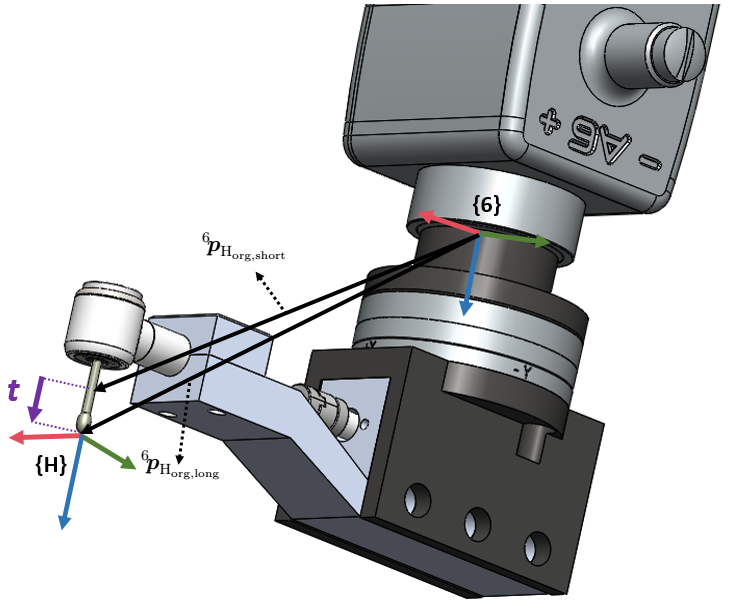
\includegraphics[width=0.7\linewidth]{Images/TCP2.png}
\caption{ 
Schematic diagram for obtaining the tool vector. 
}\label{fig:tcp2}
\end{center}
\end{figure}
Turning now to the discussion about the rotation vector. Above all, we have to find the vector of tool insertion direction $\boldsymbol{t}$. By means of TCP method, we can obtain the translation vector from the origin of frame\{6\} to the tool tip. Accordingly we use two root canal files with different lengths and apply TCP method to separately obtain two vector illustrated as Fig \ref{fig:tcp2}. Hence, 
\begin{equation}
\begin{split}
\boldsymbol{t} =\ ^\mathrm{6}\!\boldsymbol{p}_\mathrm{H_{org,long}} -\ ^\mathrm{6}\!\boldsymbol{p}_\mathrm{H_{org,short}}
\end{split}
\end{equation}
\begin{figure}[H]
\begin{center}
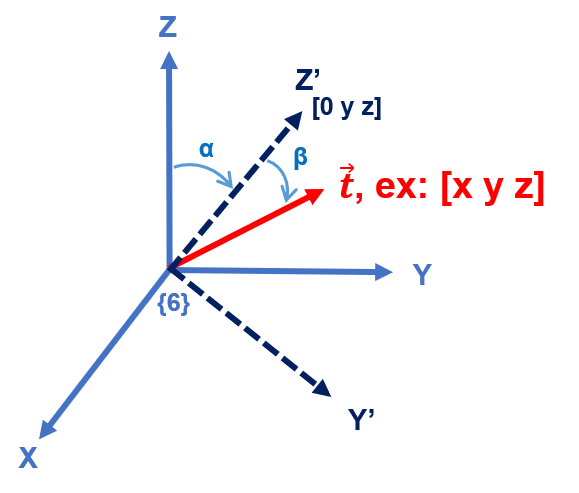
\includegraphics[width=0.6\linewidth]{Images/rot_inf.png}
\caption{
Illustration of finding the rotation matrix
}\label{fig:rot_inf}
\end{center}
\end{figure} 
For analyzing it easily, we depict it in Fig \ref{fig:rot_inf}. Note that here we only discuss rotation, so we assume that we have done translation and matched the frame\{S\} with frame\{6\}. Because we hope to send z axis command to achieve tool insertion, we should align original Z axis to the target vector. Nevertheless, Z axis alignment without other restrictions will produce many solutions. We choose one of solutions to align Z axis to the target vector. According to the figure, we assume the target vector $\boldsymbol{t}$ is $\left[x,y,z\right]$, whose projection to yz-plane $\mathrm{proj_{(y-z)}}\boldsymbol{t}$ is $\left[0,y,z\right]$. Initially, we rotate $\alpha$ degree around X axis to make original Z axis align the projection $\left[0,y,z\right]$. Next, we rotate $\beta$ degree around Y' axis and finally align original Z axis to the target vector [1,1,1]. The following equation 
\begin{equation}
\begin{split}
\ \  _{\mathrm{6}}^{\mathrm{T}}\mathbf{R} = \mathbf{R_x(\alpha)} \cdot \mathbf{R_y(\beta)}
\end{split}
\end{equation}
where
\begin{equation}
\begin{split}
\alpha &= 
-\mathrm{sign}(t_y)\cdot \cos^{-1} \left(  \frac{\hat{k}						\cdot 		\mathrm{proj_{(y-z)}}\boldsymbol{t}				}
								 				{\left \| \hat{k} \right \| 	\cdot \left \| \mathrm{proj_{(y-z)}}\boldsymbol{t} \right \|} \right)\ \\
\beta  &= 
\mathrm{sign}(t_x)\cdot \cos^{-1} \left( \frac{\textbf{t}							\cdot 		\mathrm{proj_{(y-z)}}\boldsymbol{t}			}
								  			  {\left \| \textbf{t}\right \| 	\cdot \left \| \mathrm{proj_{(y-z)}}\boldsymbol{t} \right \|} \right)\ 
\end{split}
\end{equation}
Assume $\boldsymbol{t} = [x,y,z]$,
\begin{equation}
\begin{split}
\alpha &= 
-\mathrm{sign}(y)\cdot \cos^{-1}	\left( \frac{z^2}{\sqrt{y^2+z^2}} \right) \mathrm{rad}\\
\beta  &= 
\mathrm{sign}(x)\cdot \cos^{-1} \left( \frac{y^2+z^2}{\sqrt{x^2+y^2+z^2}\sqrt{x^2+y^2+z^2}} \right) \mathrm{rad}
\end{split}
\end{equation}
$\alpha$ and $\beta$ are Euler angles, which meet the command demand.
\par
In this section, we have demonstrated two key aspects of reference frame changing of the robot arm. It's easy to input the results of section \ref{sec:tcp} and section \ref{sec:rot inf} via the command setTRF, the robot arm will recognize frame\{T\}. Having discussed how to combine a robot arm with an end effector, the next section addresses ways of combining an F/T sensor.
\chapter{Force-Guided Robot Alignment}
This chapter follows on from the previous issue about the integration, we continue to demonstrate some technical solutions of system integration. On top of that, Forces and Torques (F/T) sensor will be included to discuss. Therefore, you can see the chapter as a operating manual when you simultaneously own a robot arm, an F/T sensor and an end effector. First of all, we will explain why we need to use F/T sensor in our project in section \ref{sec:pro def}. Furthermore, we will introduce how to compensate the gravity affection while moving the robot in senction \ref{sec:grav compen}. Admittance control based on F/T sensor will be described in section \ref{sec:adm ctrl}. Coordinate transformation of F/T sensor will be interpreted in section \ref{sec:rfc}. Last but not least, we will discuss affection of setting admittance control parameters in section \ref{sec:affection}.
\section{Problem Definition}
\label{sec:pro def}
A.	Problem definition:
1. why not Image processing				2. How to cooperate with a dentist
\par\noindent
B.	Proposed method
1. Like Peg-in-hole method based on F/T feedback \cite{7743375} 	2. Two modes - Dragging mode and Self-alignment mode
\par\noindent
how to compensate the gravity affection in section \ref{sec:grav compen}; how to use admittance control in section with F/T sensor \ref{sec:adm ctrl}; and how to obtain the real force and torque values in the tool tip frame in section \ref{sec:rfc}

\section{Integration of F/T sensor}
\label{sec:grav compen}
\begin{figure}[htbp]
\begin{center}
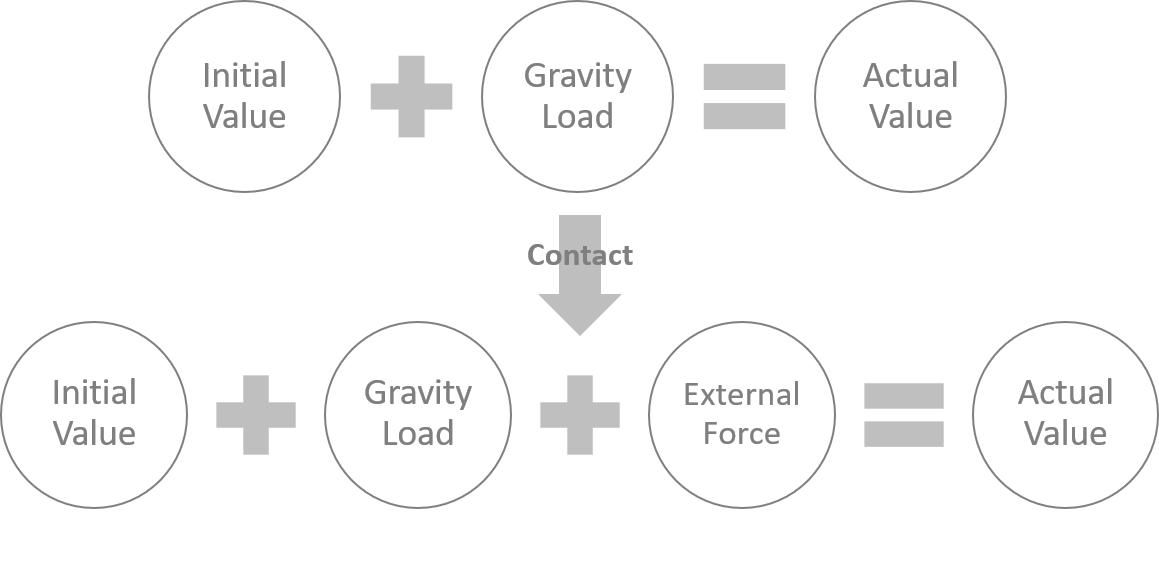
\includegraphics[width=1\linewidth]{Images/gravity compensation.png}
\caption{
Data Analysis of F/T sensor.
}\label{fig:gravity compensation}
\end{center}
\end{figure}
Gravity compensation is a critical technical issue when combining an F/T sensor with a robot arm and an end effector \cite{8997006}. 
Fundamentally, we should receive stable data when a static F/T sensor bears the same load or force. Nevertheless, our F/T sensor is installed on the robot arm and move with the pose of the robot arm. On account of its mobility, the gravity of the end effector will significantly affect the actual value we received. Moreover, starting without resetting the F/T sensor to zero would lead to an initial value. If we could not analyze the actual value to an initial value and a gravity load, we would obtain an unstable actual value, not to mention obtain the external force caused by contact force.
\par
Therefore, we illustrate a method, which is to analyze the actual value of the F/T sensor to an initial value and gravity load in real-time. It's worth noting that with this approach, we can get the installation angle between the F/T sensor and the robot arm including assembly error, and we no longer need to reset the F/T sensor to zero every time.
\subsubsection{The Centroid Position of End Effector}
To start with the first equation in Figure \ref{fig:gravity compensation},
\begin{equation}\label{eq:gc_iga}
\begin{split}
\text{Initial value}	+ \text{Gravity Load} 		= \text{Actual Value} \\
\Rightarrow \left\{\begin{matrix}
\boldsymbol{f_0}		+\boldsymbol{f_g}			&= \boldsymbol{f}\\ 
\boldsymbol{\tau_0}	+\boldsymbol{\tau_g}		&= \boldsymbol{\tau}	
\end{matrix}\right.\Rightarrow \left\{\begin{matrix}
f_{0x} 				+f_{gx} 			&= f_x\\ 
f_{0y}				+f_{gz} 			&= f_y\\ 
f_{0z}				+f_{gy} 			&= f_z\\ 
\tau_{0x}			+\tau_{gx} 			&=\tau _x\\ 
\tau_{0y}			+\tau_{gy} 			&=\tau _y \\ 
\tau_{0z}			+\tau_{gz} 			&=\tau _z 
\end{matrix}\right.	\\
\end{split}
\end{equation}
where $\boldsymbol{f}$ and $\boldsymbol{\tau}$ are force and torque vector respectively.
\par\noindent
And, by terms of moment arm formula,
\begin{equation}
\begin{split}
\because
\boldsymbol{\tau_g}	&= \boldsymbol{r} \times \boldsymbol{f_g} \\
\end{split}
\end{equation}
\par
where $\boldsymbol{r}$ denotes the centroid position of the end effector in the sensor frame.
\begin{equation}
\begin{split}
\therefore\ 
\boldsymbol{\tau}		&= \boldsymbol{\tau_0}	+\boldsymbol{\tau_g}\\
						&= \boldsymbol{\tau_0}	+
						   \boldsymbol{r} \times \boldsymbol{f_g}\\
\end{split}
\end{equation}
Then, Substitute the first line of Equation \ref{eq:gc_iga} into the above equation, we will obtain
\begin{equation}
\begin{split}
\boldsymbol{\tau}	&=  \boldsymbol{\tau_0}+ 
						\boldsymbol{p}	\times \left( \boldsymbol{f} - \boldsymbol{f_0} \right) 
\end{split}
\end{equation}
, which could be extended as
\begin{equation}
\begin{split}
\left\{\begin{matrix}
\tau _{x}	=	\tau _{0x} 	+ \left( f_z - f_{0z}\right) \cdot y - \left( f_y - f_{0y}\right) \cdot z\\
\tau _{y}	=	\tau _{0y}	+ \left( f_x - f_{0x}\right) \cdot z - \left( f_z - f_{0z}\right) \cdot x\\
\tau _{z}	=	\tau _{0z}	+ \left( f_y - f_{0y}\right) \cdot x - \left( f_x - f_{0x}\right) \cdot y& 
\end{matrix}\right.	\\
\end{split}
\end{equation}
and be overwritten as
\begin{equation}\label{eq:matrix_mfrk}
\begin{split}
\begin{bmatrix}
\tau _x\\
\tau _y\\
\tau _z
\end{bmatrix}
=
\begin{bmatrix}
0		&f_z	&-f_y	&1	&0	&0\\
-f_z	&0		&f_x	&0	&1	&0\\
f_y		&-f_x	&0		&0	&0	&1
\end{bmatrix}
\begin{bmatrix}
x\\
y\\
z\\
k_1\\
k_2\\
k_3
\end{bmatrix}\\
\end{split}
\end{equation}
\par
where
\begin{equation}\label{eq:k1k2k3}
\begin{split}
\left\{\begin{matrix}
k_1 = \tau _{0x} - \left( f_{0z} \cdot y + f_{0y} \cdot z \right)  &  \\
k_2 = \tau _{0y} - \left( f_{0x} \cdot z + f_{0z} \cdot x \right)  &\text{are all constant} \\
k_3 = \tau _{0z} - \left( f_{0y} \cdot x + f_{0x} \cdot y \right)  & 
\end{matrix}\right.\\
\end{split}
\end{equation}
With extracting $[x,y,z,k_1,k_2,k_3]$ in mind, we move the robot arm to $n\ (n\geq3)$ positions with different poses. By recording $n$ torque vectors and corresponding $n$ force vectors from F/T sensor, we can expand Equation \ref{eq:matrix_mfrk} as
\begin{equation}
\begin{split}
\begin{bmatrix}
\tau _x^1	\\
\tau _y^1	\\
\tau _z^1	\\
\tau _x^2	\\
\tau _y^2	\\
\tau _z^2	\\
\vdots\\
\tau _x^n	\\
\tau _y^n	\\
\tau _z^n	
\end{bmatrix}
=
\begin{bmatrix}
0			&f_z^1		&-f_y^1		&1	&0	&0\\
-f_z^1		&0			&f_x^1		&0	&1	&0\\
f_y^1		&-f_x^1		&0			&0	&0	&1\\
0			&f_z^2		&-f_y^2		&1	&0	&0\\
-f_z^2		&0			&f_x^2		&0	&1	&0\\
f_y^2		&-f_x^2		&0			&0	&0	&1\\
 			& 			&\vdots		& 	& 	& \\
0			&f_z^3		&-f_y^3		&1	&0	&0\\
-f_z^3		&0			&f_x^3		&0	&1	&0\\
f_y^3		&-f_x^3		&0			&0	&0	&1
\end{bmatrix}
\begin{bmatrix}
x\\
y\\
z\\
k_1\\
k_2\\
k_3
\end{bmatrix}\\
\end{split}
\end{equation}
\par
, which is defined as 
\begin{equation}
\begin{split}
\boldsymbol{m}_{\left(3n \times 1\right)} = \mathbf{F}_{\left(3n \times 6\right)} \cdot \boldsymbol{p}_{\left(6 \times 1\right)}
\end{split}
\end{equation}
As a consequence of the full column rank of $\mathbf{F}$, we can apply Moore-Penrose pseudoinverse. Then, 
\begin{equation*}
\begin{split}
\boldsymbol{p} 	&= \mathbf{F}^{\dagger} \cdot \boldsymbol{m}\\
				&= \left( \mathbf{F}^\top\mathbf{F}\right) ^{-1}\mathbf{F}^\top \cdot \boldsymbol{m}
\end{split}
\end{equation*}
\par
From now on, we have already known the centroid position of end effector in the sensor frame and values of the constants $k_1,k_2,k_3$.
\subsubsection{Gravity Compensation and Initial Value Reset}
Next, let us come back to the first equation in Figure \ref{fig:gravity compensation}. We continue to use this formula and contemplate it from the perspective of coordinate transformation relation. Here we hypothesize that the end effector weighs $g$ kilograms relative to the frame\{0\} which is also the world frame. That means the gravity vector of the end effector $\boldsymbol{^0\!g}$ is $[0,0,-g]$ in the frame\{0\}. Then, we can derive it as following.
\begin{equation}
\begin{split}
\text{Initial value}	+ \text{Gravity Load} 		&= \text{Actual Value} \\
\Rightarrow
\boldsymbol{f_0} +\  ^\mathrm{S}_6\mathbf{R} \cdot ^6_0\!\mathbf{R} \cdot \boldsymbol{^0\!g} &= \boldsymbol{f}
\end{split}
\end{equation}
\par
which is relative to frame \{6\}.
Hence, we assume an installation angle $\theta$ including assembly error.
\begin{equation}
\begin{split}
 ^\mathrm{S}_6\mathbf{R}
=
\begin{bmatrix}
\cos(\theta)	&\sin(\theta)	&0 \\
-\sin(\theta)	&\cos(\theta)	&0 \\
0				&0				&1
\end{bmatrix}
\end{split}
\end{equation}
Besides, we can easily calculate $^6_0\mathbf{R}$ from Equation \ref{eq:translation matrix}.
\begin{equation}
\begin{split}
^6_0\mathbf{R} 	&=\ ^0_6\mathbf{R}^\top\\
				&\coloneqq
\begin{bmatrix}
r_{11}		&r_{12}		&r_{13} \\
r_{21}		&r_{22}		&r_{23} \\
r_{31}		&r_{32}		&r_{33}
\end{bmatrix}
\end{split}
\end{equation}
Therefore,
\begin{equation}
\begin{split}
\begin{bmatrix}
f_{0x}\\
f_{0y}\\
f_{0z}
\end{bmatrix}
+
\begin{bmatrix}
\cos(\theta)	&\sin(\theta)	&0 \\
-\sin(\theta)	&\cos(\theta)	&0 \\
0				&0				&1
\end{bmatrix}
\begin{bmatrix}
r_{11}		&r_{12}		&r_{13} \\
r_{21}		&r_{22}		&r_{23} \\
r_{31}		&r_{32}		&r_{33}
\end{bmatrix}
\begin{bmatrix}
0\\
0\\
-g
\end{bmatrix}
=
\begin{bmatrix}
f_x\\
f_y\\
f_z
\end{bmatrix}
\end{split}
\end{equation}
\par
Further, we rewrite it as 
\begin{equation}
\label{eq:matrix_rgf0f}
\begin{split}
\begin{bmatrix}
-r_{13}		&-r_{23} 	&0			&1		&0		&0\\
-r_{23}		&r_{13}		&0			&0		&1		&0\\
0			&0			&-r_{33}	&0		&0		&1
\end{bmatrix}
\begin{bmatrix}
g\cos(\theta)\\
g\sin(\theta)\\
g\\
f_{0x}\\
f_{0y}\\
f_{0z}
\end{bmatrix}
=
\begin{bmatrix}
f_x\\
f_y\\
f_z
\end{bmatrix}
\end{split}
\end{equation}
In the same way as Equation \ref{eq:matrix_mfrk}, we can extract $[g\cos(\theta),g\sin(\theta),g,f_{0x},f_{0y},f_{0z}]$ by the least square solution. Note that, we can simultaneously record these data when using the method in Equation \ref{eq:matrix_mfrk}. By recording $n(n\geq3)$ third columns of ration matrices and corresponding $n$ force vectors from F/T sensor, we can expand Equation \ref{eq:matrix_rgf0f} as
\begin{equation}
\begin{split}
\begin{bmatrix}
-r_{13}^1		&-r_{23} ^1		&0			&1		&0		&0\\
-r_{23}^1		&r_{13}^1		&0			&0		&1		&0\\
0				&0				&-r_{33}^1	&0		&0		&1\\
-r_{13}^2		&-r_{23}^2 		&0			&1		&0		&0\\
-r_{23}^2		&r_{13}^2		&0			&0		&1		&0\\
0				&0				&-r_{33}^2	&0		&0		&1\\
&&\vdots\\
-r_{13}^n		&-r_{23}^n 		&0			&1		&0		&0\\
-r_{23}^n		&r_{13}^n		&0			&0		&1		&0\\
0				&0				&-r_{33}^n	&0		&0		&1
\end{bmatrix}
\begin{bmatrix}
g\cos(\theta)\\
g\sin(\theta)\\
g\\
f_{0x}\\
f_{0y}\\
f_{0z}
\end{bmatrix}
=
\begin{bmatrix}
f^1_{0x}\\
f^1_{0y}\\
f^1_{0z}\\
f^2_{0x}\\
f^2_{0y}\\
f^2_{0z}\\
\vdots\\
f^n_{0x}\\
f^n_{0y}\\
f^n_{0z}
\end{bmatrix}
\end{split}
\end{equation}
\par
, which is defined as 
\begin{equation}
\begin{split}
\mathbf{M}_{\left(3n \times 6\right)} \cdot \boldsymbol{p}_{\left(6 \times 1\right)} = \boldsymbol{f}_{\left(3n \times 1\right)}
\end{split}
\end{equation}
As a consequence of the full column rank of $\mathbf{M}$, we can apply Moore-Penrose pseudoinverse. Then, 
\begin{equation*}
\begin{split}
\boldsymbol{p} 	&= \mathbf{M}^{\dagger} \cdot \boldsymbol{f}\\
				&= \left( \mathbf{M}^\top\mathbf{M}\right) ^{-1}\mathbf{M}^\top \cdot \boldsymbol{f}
\end{split}
\end{equation*}
Apparently, we can directly obtain $g,f_{0x},f_{0y},f_{0z}$. Afterwards, we substitute them into Equation \ref{eq:k1k2k3} to calculate 
\begin{equation}
\begin{split}
\left\{\begin{matrix}
\tau _{0x}	=	k_1	+ \left( f_{0z} \cdot y + f_{0y} \cdot z \right) \\
\tau _{0y} 	=	k_2	+ \left( f_{0x} \cdot z + f_{0z} \cdot x \right) \\
\tau _{0z} 	=	k_3 + \left( f_{0y} \cdot x + f_{0x} \cdot y \right)
\end{matrix}\right.\\
\end{split}
\end{equation}
Finally, we successfully obtain the weight of the end effector $g$, the initial value of the F/T sensor $[f_{0x},f_{0y},f_{0z},\tau_{0x},\tau_{0y},\tau_{0z}]$.
\par
As for installation angle $\theta$ including assembly error,  there is an further discussion. Undoubtedly, we can derive it as
\begin{equation}
\begin{split}
\theta = \cos^{-1}\left(\frac{g\cos(\theta)}{g}\right)\ \text{or} \ \sin^{-1}\left(\frac{g\sin(\theta)}{g}\right)\
\end{split}
\end{equation}
In theory, By either arccos function or arcsin function we can derive the same value. However, we estimate $[g\cos(\theta),g\sin(\theta),g,f_{0x},f_{0y},f_{0z}]$ by using the least square solution which produce a approximated answer rather than the correct answer. A subtle bias caused by the least square solution will be enlarged through the arc function. 
Thankfully, we originally designed an adapter to connect the robot arm and F/T sensor and the installation angle is exactly zero degree. Therefore, here we only need to concern about the subtle bias result from assembly errors.\\
Here we take the same bias and compare arccos to arcsin. 
\begin{table}[htbp]
\centering
\caption{Arc-function Comparison}
\label{tab:arc}
\begin{tabular}{c|c|c} 
\hline \hline
bias $n$ (rad)	&$\sin^{-1}(n)$	(degree)	&$\cos^{-1}(1-n)$ (degree)\\
\hline
0				&0							&0\\
0.001			&0.057						&2.56\\
0.01			&0.57						&8.11\\
0.1				&5.7						&25.84
\end{tabular}
\end{table}
Obviously, if we separately give the same bias ( $0.1$ rad) into arccos and arcsin function, arccos function will enlarge the bias significantly larger than arcsin function. Hence we should use
\begin{equation}
\begin{split}
\theta = \sin^{-1}\left(\frac{g\sin(\theta)}{g}\right)\
\end{split}
\end{equation}
Notably, as a result of the zero installation angle which we originally designed, from Table \ref{tab:arc} we could infer to use arcsin function. In contrast, if the installation angle is not zero, the above assumption will be invalid.
\par
Ultimately, we have successfully dissected the actual value of F/T sensor into the initial value of F/T sensor and the gravity of the end effector. 
\subsubsection{External Force Evaluation}
Next, we continue to review the second equation in  Figure \ref{fig:gravity compensation}.
\begin{equation}
\begin{split}
\text{Initial value}	+ \text{Gravity Load} 		+ \text{External Force}		&= \text{Actual Value} \\
\Rightarrow \left\{\begin{matrix}
\boldsymbol{f_0}		+\boldsymbol{f_g}		+\boldsymbol{f_e}		&= \boldsymbol{f}\\ 
\boldsymbol{\tau_0}		+\boldsymbol{\tau_g}	+\boldsymbol{\tau_e}		&= \boldsymbol{\tau}	
\end{matrix}\right.	\\
\end{split}
\end{equation}
Therefore,
\begin{equation}
\begin{split}
\boldsymbol{f_e}		&= \boldsymbol{f} 		- \boldsymbol{f_0}		-\boldsymbol{f_g}\\
						&= \boldsymbol{f} 		- \boldsymbol{f_0}		- ^\mathrm{S}_6\mathbf{R} \cdot ^6_0\!\mathbf{R} \cdot \boldsymbol{^0\!g}\\
\boldsymbol{\tau_e}		&= \boldsymbol{\tau}	- \boldsymbol{\tau_0}		-\boldsymbol{\tau_g}\\
						&= \boldsymbol{\tau}	- \boldsymbol{\tau_0}		-\boldsymbol{r} \times \boldsymbol{f_g}
\end{split}
\end{equation}
\begin{equation*}
\begin{split}
\Rightarrow 
\left\{\begin{matrix}
f_{ex} = f_x - f_{0x} 	+ g\cos(\theta)r_{13} 	+ g\sin(\theta)r_{23}\\
f_{ey} = f_y - f_{0y} 	- g\sin(\theta)r_{13} 	+ g\cos(\theta)r_{23}\\
f_{ez} = f_z - f_{0z} 	+ gr_{33}\\
\tau_{ex} = f_x - \tau_{0x} - \left( g_z\cdot y - g_y\cdot z \right)\\
\tau_{ey} = f_y - \tau_{0y} - \left( g_x\cdot z - g_z\cdot x \right)\\
\tau_{ez} = f_z - \tau_{0z} - \left( g_y\cdot x - g_x\cdot y \right)
\end{matrix}\right.
\end{split}
\end{equation*}
\section{Dragging Mode}
In the hope that dentist could drag our system to an infected tooth by holding the end effector, we usher in admittance control based on F/T sensor.
\subsection{Admittance Control based on F/T sensor}
\label{sec:adm ctrl}
\subsubsection{Control Scheme}
Admittance control make the robot move like a spring-mass-damper system. Forces and torques can be mapped into the movements such as position or velocity. Most important of all, admittance control enables an robot arm to cooperate with human in a safe work environment.Since Meca500 is an industrial robot arm without admittance control, we subsequently combine the robot arm with the F/T sensor so as to adopt admittance control. With force and torque feedback, F/T sensor make Meca500 be resemble to a collaborative robot arm. Therefore, we propose a control scheme depicted as Figure \ref{fig:adm ctrl}. It's worth noting that in this approach the admittance control function is triggered by the end effector mounted on F/T sensor instead of detecting each wrist torque of the robot arm.
\par
\begin{figure}[htbp]
\begin{center}
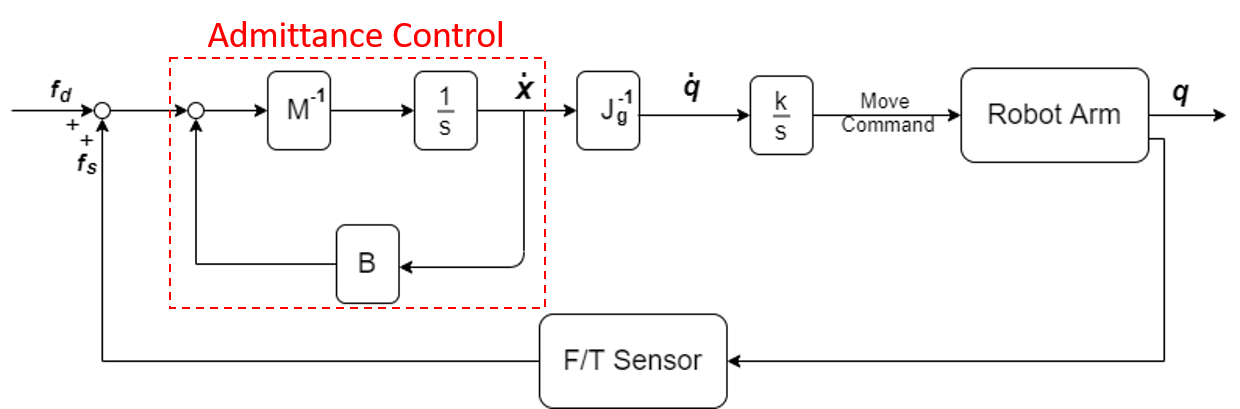
\includegraphics[width=1\linewidth]{Images/adm ctrl.png}
\caption{
Control scheme. $\boldsymbol{f_d}$ denotes the desired forces and torques vector. $\boldsymbol{f_s}$ denotes the real value detected by F/T sensor and is also a forces and torques vector. $\boldsymbol{\dot{x}}$ denotes [$\dot{x}, \dot{y}, \dot{z}, \dot{\theta _x}, \dot{\theta _y}, \dot{\theta _z}$]. $\mathbf{J_g}$ denotes the geometric Jacobian matrix. $\boldsymbol{\dot{q}}$ denotes [$\dot{\theta _1}, \dot{\theta _2}, \dot{\theta _3}, \dot{\theta _4}, \dot{\theta _5}, \dot{\theta _6}$]. $\boldsymbol{q}$ denotes $\left[\theta _1, \theta _2, \theta _3, \theta _4, \theta _5, \theta _6 \right] $.
}\label{fig:adm ctrl}
\end{center}
\end{figure}
\par
A standard equation of admittance control is represented as Equation \ref{eq:adm_mbk}. The values we obtain from the F/T sensor are $\left[f_x, f_y, f_z,\tau _x, \tau _y, \tau _z \right]$, whose forces $ \left[f_x, f_y, f_z\right]$ are related to the translations $ \left[x, y, z\right]$ and torques $ \left[\tau _x, \tau _y, \tau _z\right]$ are related to the axis angle $ \left[\theta _x,\theta _y,\theta _z\right]$. 
\begin{equation}
\label{eq:adm_mbk}
\begin{split}
\begin{bmatrix}
x \\
y \\
z \\
\theta _x \\
\theta _y \\
\theta _z 
\end{bmatrix}
=
\frac{1}{\mathbf{M}\mathrm{S}^2+\mathbf{B}\mathrm{S}+\mathbf{K}}
\begin{bmatrix}
f_x \\
f_y \\
f_z \\
\tau _x \\
\tau _y \\
\tau _z 
\end{bmatrix}
\end{split}
\end{equation}
\subsubsection{Selection of Admittance Control Model}
In our proposed approach we omit parameter $\mathbf{K}$ which is relevant to spring stiffness, considering that it's not necessary to bounce such as a spring. Therefore, our system should behave like a mass-damper system as following.
\begin{equation}
\label{eq:adm_mb}
\begin{split}
\begin{bmatrix}
x \\
y \\
z \\
\theta _x \\
\theta _y \\
\theta _z 
\end{bmatrix}
=
\frac{1}{\mathbf{M}\mathrm{S}^2+\mathbf{B}\mathrm{S}}
\begin{bmatrix}
f_x \\
f_y \\
f_z \\
\tau _x \\
\tau _y \\
\tau _z 
\end{bmatrix}
\end{split}
\end{equation}
where $\mathbf{M},\mathbf{B},\mathbf{K}$ are diagonal positive definite matrices. Affections of these parameters will be discussed in section \ref{sec:affection}.
\subsubsection{Robot Command Decision}
After determining our admittance control model, we should select a correspondent command to move the robot. However there are many commands of moving the robot arm, as shown in Table \ref{tab:commands}.
\begin{table}[htbp]
\centering
\caption{Moving commands in Meca500}
\label{tab:commands}
\begin{tabular}{c|c|l} 
\hline \hline
Types										&Commands			&Input parameters\\
\cline{1-3}
\multirow{2}{*}{Position}					&MoveJoints			&\noindent $\theta _1, \theta _2 ,\theta _3 ,\theta _4 ,\theta _5 , \theta _6 $\\\cline{2-3}
											&MovePose			&\noindent$x,y,z,\alpha ,\beta ,\gamma $\\
\cline{1-3}
\multirow{2}{*}{Velocity}					&MoveJointsVel		&$\dot{\theta}_1, \dot{\theta}_2, \dot{\theta}_3,\dot{\theta}_4, \dot{\theta}_5 , \dot{\theta}_6 $\\\cline{2-3}
											&MoveLinVelTRF		&$\dot{x},\dot{y},\dot{z},\dot{\theta _x},\dot{\theta _y},\dot{\theta _z}$\\
\hline \hline
\end{tabular}
\end{table}
\par
Considering that the singularity problem is an imperative problem in robotics, we intend to use MoveJoints or MoveJointsVel to directly set the angles of axis. Despite that it's easier to implement admittance control via other commands, the system would touch the singularity point at any time. It undoubtedly expose patients to danger because the uncertainty of the system. Therefore, position command - MoveJoints and velocity command - MoveJointsVel is our options. Why we choose the command MoveJoints  is that Meca500 has a default time-out value to essure its safty. Despite we could set this value from 0.001 to 2 second, Meca500 is still restricted to move with this value. For example, the value of time-out is set $0.1$ sec. While the robot receive a command, the robot move for $0.1$ sec then immideatly stop. It's not easy to control via velocity command due to this default property.
\par
Finally, we designate MoveJointsVel $\left(\dot{\theta}_1, \dot{\theta}_2,\cdots , \dot{\theta}_6 \right)$ as our main command. Thanks to the property of Jacobian matrix shown in Equation \ref{eq:jg6}, we can transform $\boldsymbol{\dot{x}}$ into $\boldsymbol{\dot{q}}$. Then we multiply it an integrator $\frac{1}{\mathrm{S}}$
to obtain $\boldsymbol{q}$. Note that, As F/T sensor is mounted on the frame\{6\}, we should use Equation \ref{eq:jg6} rather than Equation \ref{eq:jg0}. 
\section{Self-Alignment Mode}
The purpose of this section is developing a framework for robot self-alignment regarding the position and orientation of root canal, which is one of the main contributions of the thesis. This function assists endodontists to automatically operate the cleaning procedure and ensures a postoperative recovery for patients. The main idea is to amend the direction of insertion by itself to lower the contact resistance.
\par
We propose a complete robotic procedure. First and foremost, the main role of this procedure is the root canal reamer. We rotate the root canal reamer to clean a pulp, move it to do reciprocation and self-alignment. All of things we care about are all on the root canal such as it position, orientation , rotation speed and contact force. Nevertheless, the robot arm and the F/T sensor have their own coordinates initially. They originally recognize its own coordinate rather than the root canal reamer's frame, so they do their work themselves respectively. Therefore, we need to let them understand the tool frame. Thanks to section \ref{sec:ref_robot}, we have demonstrated how to change the reference frame of the robot arm. After that, we are capable of identifying the translation and rotation information of the root canal reamer and subsequently obtaining the transformation matrix from the robot arm to the tool. As for F/T sensor, we have explained how to do gravity compensation in section \ref{sec:grav compen}, we will interpret how to change its fiducial to the tool tip in section \ref{sec:rfc}. Besides, we will advance a motion planning in accordance with dentist's motion and standard surgical solution in section \ref{sec:motion planning} 
\subsection{Coordinate Transformation of F/T sensor}
\label{sec:rfc}
Similar to Coordinate transformation of F/T sensor in section \ref{sec:ref_robot}. The F/T sensor originally recognize its own coordinate rather than the root canal reamer's frame. Namely, F/T sensor receives unmatched data when the tool contacts an obstacle due to the wrong reference frame. Hence, here we illustrate how to obtain the coordinate transformation of F/T sensor so as to decouple the force and toque from frame\{S\} to the frame\{T\}. We analyze it in two perspective - reference frame changing and measurement point changing.
\par
\begin{figure}[htbp]
\begin{center}
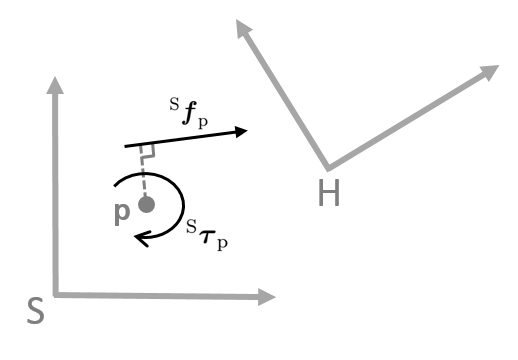
\includegraphics[width=0.7\linewidth]{Images/sensor_comp 1.png}
\caption{
Illustration of changing reference frame from $\{\mathrm{S}\} $ to $\{\mathrm{T}\}$. $\mathrm{f}$ and $\mathrm{m}$ respectively denote a force and a moment measured at point p.
}\label{fig:sensor_comp1}
\end{center}
\end{figure}
\par\noindent
In view of reference frame changing in Figure \ref{fig:sensor_comp1}, we can derive the following equation.
\begin{equation}
\begin{split}
\begin{bmatrix}
\boldsymbol{f}_\mathrm{p}\\ 
\boldsymbol{m}_\mathrm{p}
\end{bmatrix}
_{\{ \mathrm{T}\}}
=
\begin{bmatrix}
_\mathrm{S}^\mathrm{T}\mathbf{R} & \boldsymbol{0}\\ 
\boldsymbol{0} & _\mathrm{S}^\mathrm{T}\mathbf{R}
\end{bmatrix}
\begin{bmatrix}
\boldsymbol{f}_\mathrm{p}\\ 
\boldsymbol{m}_\mathrm{p}
\end{bmatrix}
_{\{ \mathrm{S}\}}
\end{split}
\end{equation}
\par
\begin{figure}[htbp]
\begin{center}
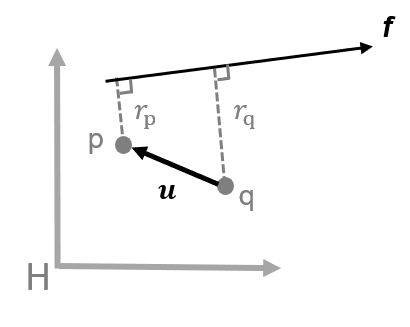
\includegraphics[width=0.7\linewidth]{Images/sensor_comp 2.png}
\caption{
Illustration of changing reference frame from $\{\mathrm{S}\} $ to $\{\mathrm{T}\}$. $\boldsymbol{f}$ and $\boldsymbol{m}$ respectively denote a force and a moment measured at point p.
}\label{fig:sensor_comp2}
\end{center}
\end{figure}
\par\noindent
On the other hand, in Figure \ref{fig:sensor_comp2} we describe a force and a torque observed in the same frame but different point.
\begin{equation}
\begin{split}
\boldsymbol{f}				&= \boldsymbol{f}_\mathrm{p} = \boldsymbol{f}_\mathrm{q}\\
\boldsymbol{m}_\mathrm{q} 	&= \boldsymbol{r}_\mathrm{q} \cdot \boldsymbol{f}\\
			 				&= \boldsymbol{r}_\mathrm{p} \cdot \boldsymbol{f}+\overrightarrow{\mathrm{q}\mathrm{p}} \times \boldsymbol{f}_\mathrm{p}\\
			 				&= \boldsymbol{m}_\mathrm{p} + \overrightarrow{\mathrm{q}\mathrm{p}}\times \boldsymbol{f}_\mathrm{p}
\end{split}
\end{equation}
Assume
\begin{equation*}
\begin{split}
\overrightarrow{\mathrm{q}\mathrm{p}}
=
\begin{bmatrix}
u_1\\
u_2\\
u_3
\end{bmatrix}
\end{split}
\end{equation*}
then
\begin{equation}
\begin{split}
\overrightarrow{\mathrm{q}\mathrm{p}}\times \boldsymbol{f}_\mathrm{p}
=
\begin{bmatrix}
0		&-u_3		&u_2		\\
u_3		&0			&-u_1		\\
-u_2	&u_1		&0		
\end{bmatrix}
\begin{bmatrix}
f_1\\
f_2\\
f_3
\end{bmatrix}
\end{split}
\end{equation}
As s result, we consider reference frame changing and measurement point changing, then we can obtain the following essential equation.
\begin{equation}
\begin{split}
\begin{bmatrix}
\boldsymbol{f}_\mathrm{q}\\ 
\boldsymbol{m}_\mathrm{q}
\end{bmatrix}
_{\{ \mathrm{T}\}}
=
\begin{bmatrix}
\mathbf{I}_{3 \times 3} & \boldsymbol{0}\\ 
\begin{matrix}
0		&-u_3		&u_2		\\
u_3		&0			&-u_1		\\
-u_2	&u_1		&0		
\end{matrix} & \mathbf{I}_{3 \times 3}
\end{bmatrix}
\begin{bmatrix}
_\mathrm{S}^\mathrm{T}\mathbf{R} & \boldsymbol{0}\\ 
\boldsymbol{0} & _\mathrm{S}^\mathrm{T}\mathbf{R}
\end{bmatrix}
\begin{bmatrix}
\boldsymbol{f}_\mathrm{p}\\ 
\boldsymbol{m}_\mathrm{p}
\end{bmatrix}
_{\{ \mathrm{S}\}}
\end{split}
\end{equation}
\subsection{Motion Planning: Based on Admittance Control}
\label{sec:motion planning} 
\begin{figure}[htbp]
\begin{center}
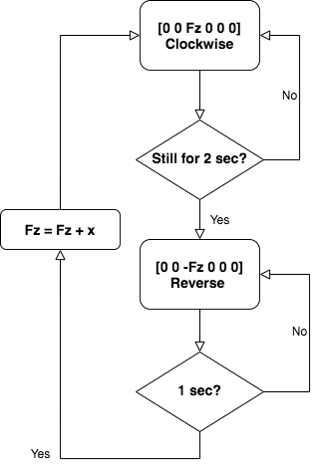
\includegraphics[width=0.5\linewidth]{Images/motion planning_flow chart.png}
\caption{
Flow chart of motion planning
}\label{fig:motion planning_flow chart}
\end{center}
\end{figure}
\begin{figure}[htbp]
\begin{center}
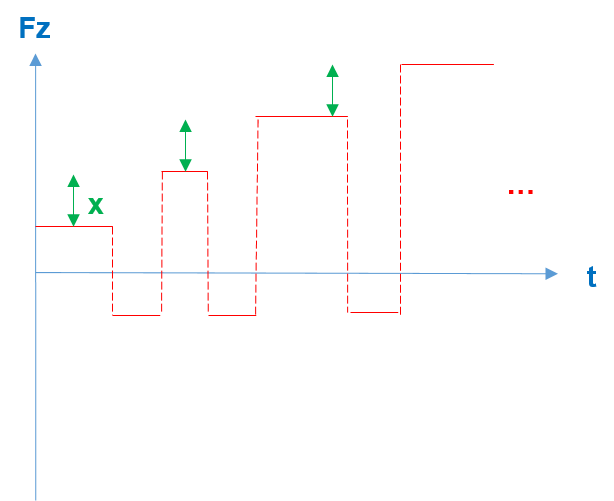
\includegraphics[width=0.5\linewidth]{Images/motion planning_motion.png}
\caption{
Flow chart of motion planning
}\label{fig:motion planning_motion}
\end{center}
\end{figure}
\section{Affections of Parameters Setting}
\label{sec:affection}
Because our system is similar to a mass- damper system, we focus on the performance of the velocity $\boldsymbol{\dot{x}}$ whereby the system could be considered as
\begin{figure}[htbp]
\begin{center}
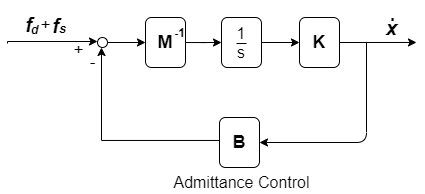
\includegraphics[width=0.6\linewidth]{Images/mass spring.png}
\end{center}
\caption{
Control scheme. $\mathbf{M},\mathbf{B},\mathbf{K}$ are all diagonal positive definite matrices, whose diagonal indexes are respectively related to $x,y,z,\theta_x,\theta_y,\theta_z$. $\mathbf{M},\mathbf{B}$ are related to the inertial and damping respectively, and $\mathbf{K}$ is a proportional gain. 
}\label{fig:mass spring}
\end{figure}
\par\noindent
It is a first-order control system and its step response is 
\begin{equation}
\begin{split}
\mathcal{L}^{-1} \left[ \frac{1}{\mathrm{S}} \cdot \frac{\mathbf{K}}{\mathbf{M}\mathrm{S}+\mathbf{B}} \right] 
&= \mathcal{L}^{-1} \left[ \frac{\mathbf{K}}{\mathbf{B}} \left( \frac{1}{\mathrm{S}} - \frac{1}{\mathrm{S}+\frac{\mathbf{B}}{\mathbf{M}}} \right) \right] \\
&= \frac{\mathbf{K}}{\mathbf{B}} \left(1 - e^{- \frac{\mathbf{B}}{\mathbf{M}} t}  \right)
\end{split}
\end{equation}
From the above derivation, we can know 
\begin{equation}
\begin{split}
\text{time constant } \mathbf{T} = \frac{\mathbf{M}}{\mathbf{B}}
\end{split}
\end{equation}
Hence,the transient response can be derived as 
\begin{equation}
\begin{split}
&\text{Rise time} = 2.3\mathbf{T} = \frac{2.3 \mathbf{M}}{\mathbf{B}}\\
&\text{Settling time} = 4\mathbf{T} =  \frac{4 \mathbf{M}}{\mathbf{B}}\\
\end{split}
\end{equation}
when $\mathrm{T}$ is larger, the pole is farer from origin in $\mathrm{S}$ domain, the system is more stable. Besides, when $\mathbf{T}$ is larger, the response speed is faster. Furthermore, we coarse-tune parameter $\mathbf{K}$ to adjust the whole gain of the system and determine the mode of the system is "Dragging Mode" or "Self-Alignment Mode". Last but not least, we fine-tune diagonal parameters of $\mathbf{B}$ separately because the inertial and spring properties of each axis are discrepant
\par
In practice, we set $(\mathbf{M} : \mathbf{B} = 1 : 1000)$  to make $(\mathbf{T} = \frac{\mathbf{M}}{\mathbf{B}} = 0.001)$, then the system rises up to $98\%$ after $0.003$ second. Further,. In Table \ref{tab: para_adm}, where $\mathbf{K} = \text{diag}(k,k,k,k,k,k)$, $\mathbf{B} = \text{diag}(b_1,b_2,b_3,b_4,b_5,b_6)$, we show detailed parameters with "Dragging Mode" and "Self-Alignment Mode".
\begin{table}[htbp]
\centering
\caption{Parameters setting of Admittance control.}
\label{tab: para_adm}
\begin{tabular}{c|c|c} 
\hline \hline
			&Dragging Mode		&Self-Alignment Mode	\\
\hline
k			&$1200$				&$500$					\\
$b_1$		&$0.4$				&$1.2$					\\
$b_2$		&$0.4$				&$0.6$					\\
$b_3$		&$0.4$				&$1.1$					\\
$b_4$		&$0.8$				&$1.7$					\\
$b_5$		&$0.8$				&$4$					\\
$b_6$		&$0.8$				&$1.8$					\\
%$m_1$		&$0.004$			&$0.012$				\\
%$m_2$		&$0.004$			&$0.006$				\\
%$m_3$		&$0.004$			&$0.011$				\\
%$m_4$		&$0.008$			&$0.017$				\\
%$m_5$		&$0.008$			&$0.04$					\\
%$m_6$		&$0.008$			&$0.018$		
\hline\hline			
\end{tabular}
\end{table}

\chapter{Control of Endodontic File Rotation}
\section{Problem Definition}
(Main cause of Files Fracture)					
\par\noindent
(File property)
\section{The Proposed Method and Theorem}
(CACS2020 Prototype 1)							
\par\noindent
(Motion Planning: sections)(Current threshold setting)
\par\noindent
Once the current of the file is in excess of the threshold, it will inversely rotate to release torque. A decline(decrease/increase/drop) in the current of the motor is indicative of contact resistance of the file.
\chapter{Preliminary Experiment Result}
\section{Experimental Setup}
(Communication protocol – EtherCAT, RTOS – NI target)						\\
For 6.2 experiment: (Stewart-Platform + PhaseSpace + markers)				\\
For 6.3 6.4 experiments: (Acrylic root canal model + truth tooth)
\section{Admittance Control}
(Metrics: position comparison between the target and the robot)
\section{Automatically Direction Changing}
(Metrics: time, completeness and file breakage)								\\
(Completeness definition: comparison of pixel area before and after experiment via image)
\section{Repetitive Experiment}
(Metrics: file breakage, compare with and without reverse)
\chapter{Conclusions and Future works}
\hspace*{6mm}An endodontic treatment is a challenging surgery for dentists due to complex conditions of teeth. Therefore, building a robot-assisted system for the endodontic robot requires comprehensive consideration on whole surgery procedures. Review the section \ref{sec:contributions}, we advocated the four parts of the project prospect. We highlight two main parts of the prospect and have proved the feasibility of our proposed approaches. The whole work of the thesis is concluded in this chapter.
\section{Conclusions}
\hspace*{6mm}Nowadays, despite that there are more and more dental robots springing up, there are still few teams specific to endodontic treatment. In view of this, our team has built the robot-assisted system, Dentibot, composed of a 6-DoF robot arm, a 6-DoF F/T sensor, and a modified handpiece. Integration issues between the above devices are reviewed and solved. The DentiBot can assist dentists in performing endodontic treatment as a consequence of the following functions. 
\par
Admittance control is ushered in to enable the dentist to move the DentiBot above an infected tooth. Also, a framework based on admittance control for robot alignment regarding the position and orientation of the root canal is presented. "Dragging Mode" and "Self-Alignment Mode" are separately implemented for the above functions.
\par
Last but not least, instrument fracture is a serious problem for dentists. It will even lead to a medical dispute. With the torque monitoring system, file feedrate control is applied to reduce the possibility of instrument fracture. 
\par
Experiments indicated that the above functions had good performances on force-guided alignment and file feedrate control. It has proven the feasibility in technical and clinical perspectives. Undoubtedly, the DentiBot can help dentists perform better clinical results.
\section{Discussion and Future Works}
\hspace*{6mm}The thesis is the pioneer of the endodontic project. Despite that the thesis develops the DentiBot and presents the above functions, there are undoubtedly some works that remained and rooms for improvement on the modified hardware and functions. The modified handpiece made by 3D-print is not durable for time-consuming endodontic treatment. It is necessary to do machining for more stable results. 
\par 
In the thesis, we hypothesize that a dentist moves the DentiBot above the root, then the DentiBot does the "Cleaning" procedure. However, sometimes there is not only one root in the tooth. For instance, there are three to four roots in molars. Therefore, we wish that the DentiBot will have the ability to search all root canals after the dentist moves the DentiBot above the infected tooth. 
\par
On top of that, we proposed the alignment method while the DentiBot does drilling. It not only aligns with the root path but also with patient moving. However, the patient tracking belongs to a minor range movement. Therefore, the DentiBot is expected to be applied to patient tracking with large movement via string potentiometers in the future.			
\chapter*{Appendix}
\addcontentsline{toc}{chapter}{Appedix}  
\section*{Appendix A \quad Forward Kinematics}
\label{appendix:forward}
\addcontentsline{toc}{section}{A \quad Forward Kinematics}  
\begin{equation*}
\begin{split}
^0_6 \mathbf{T} =
^0_1 \mathbf{T} \cdot ^1_2 \mathbf{T} \cdot ^2_3 \mathbf{T} \cdot ^3_4 \mathbf{T} \cdot ^4_5 \mathbf{T} \cdot ^5_6 \mathbf{T} =
\begin{bmatrix}
^0_6 \mathbf{R}_{3\times 3} 	&^0\!\boldsymbol{p}_\mathrm{6_{org}}\\
0_{1\times 3}				&1\\
\end{bmatrix}
=
\begin{bmatrix}
t_{11} 	&t_{12}	&t_{13}	& t_{14}\\
t_{21} 	&t_{22}	&t_{23}	& t_{24}\\
t_{31} 	&t_{32}	&t_{33}	& t_{34}\\
0					&0					&0					&1\\
\end{bmatrix}
\end{split}
\end{equation*}
$t_{11} =\	- S_6(C_4S_1 + S_4(C_1S_3-C_2 - C_1C_3S_2)) - C_6(C_5(S_1S_4 - C_4(C_1S_3\\
			-C_2 - C_1C_3S_2)) - S_5(C_1C_3-C_2 + C_1S_2S_3))$\\
$t_{12} =\ 	S_6(C_5(S_1S_4 - C_4(C_1S_3-C_2 - C_1C_3S_2)) - S_5(C_1C_3-C_2 + C_1S_2S_3))\\
		 	- C_6(C_4S_1 + S_4(C_1S_3-C_2 - C_1C_3S_2))$\\
$t_{13} =\ 	- S_5(S_1S_4 - C_4(C_1S_3-C_2 - C_1C_3S_2)) - C_5(C_1C_3-C_2 + C_1S_2S_3)$\\
$t_{14} =\ 	135C_1S_2 - 70S_5(S_1S_4 - C_4(C_1S_3-C_2 - C_1C_3S_2)) - 70C_5(C_1C_3-C_2\\
		 	+ C_1S_2S_3) - 120C_1C_3-C_2 - 120C_1S_2S_3 - 38C_1S_3-C_2 + 38C_1C_3S_2$\\
$t_{21} =\ 	S_6(C_1C_4 + S_4(C_3S_2S_1 - S_1S_3-C_2)) + C_6(C_5(C_1S_4 - C_4(C_3S_2S_1\\
		 	- S_1S_3-C_2)) + S_5(C_3S_1-C_2 + S_2S_1S_3))$\\
$t_{22} =\ 	C_6(C_1C_4 + S_4(C_3S_2S_1 - S_1S_3-C_2)) - S_6(C_5(C_1S_4 - C_4(C_3S_2S_1\\
		 	- S_1S_3-C_2)) + S_5(C_3S_1-C_2 + S_2S_1S_3))$\\
$t_{23} =\ 	S_5(C_1S_4 - C_4(C_3S_2S_1 - S_1S_3-C_2)) - C_5(C_3S_1-C_2 + S_2S_1S_3)$\\
$t_{24} =\ 	135S_2S_1 + 70S_5(C_1S_4 - C_4(C_3S_2S_1 - S_1S_3-C_2)) - 70C_5(C_3S_1-C_2\\
		 	+ S_2S_1S_3) + 38C_3S_2S_1 - 120C_3S_1-C_2 - 120S_2S_1S_3 - 38S_1S_3-C_2$\\
$t_{31} =\ 	C_6(S_5(C_3S_2 - S_3-C_2) + C_4C_5(C_3-C_2 + S_2S_3)) - S_4S_6(C_3-C_2\\
			+ S_2S_3)$\\
$t_{32} =\ 	- S_6(S_5(C_3S_2 - S_3-C_2) + C_4C_5(C_3-C_2 + S_2S_3)) - C_6S_4(C_3-C_2\\
		 	+ S_2S_3)$\\
$t_{33} =\ 	C_4S_5(C_3-C_2 + S_2S_3) - C_5(C_3S_2 - S_3-C_2)$\\
$t_{34} =\ 	120S_3-C_2 - 120C_3S_2 - 38C_3-C_2 - 38S_2S_3 - 135-C_2\\
			- 70C_5(C_3S_2 - S_3-C_2) + 70C_4S_5(C_3-C_2 + S_2S_3) + 135$


\section*{Appendix B \quad Jacobian Matrix}
\label{appendix:jacobian}
\addcontentsline{toc}{section}{B \quad Jacobian Matrix }  
\subsection*{Jg0}
$j_{g0,21} =\  135C_1S_2 - 120C_1S_2S_3 - 70S_1S_4S_5 + 120C_1C_2C_3 + 38C_1C_2S_3\\
			   + 38C_1C_3S_2 + 70C_1C_2C_3C_5 - 70C_1C_5S_2S_3 - 70C_1C_2C_4S_3S_5\\
		 	   - 70C_1C_3C_4S_2S_5$\\
$j_{g0,22} =\  -S_1(120C_2S_3 - 38C_2C_3 - 135C_2 + 120C_3S_2 + 38S_2S_3 + 70C_2C_5S_3\\
		   	   + 70C_3C_5S_2 + 70C_2C_3C_4S_5 - 70C_4S_2S_3S_5)$\\
$j_{g0,23} =\  -2S_1(60C_2S_3 - 19C_2C_3 + 60C_3S_2 + 19S_2S_3 + 35C_2C_5S_3\\
			   + 35C_3C_5S_2 + 35C_2C_3C_4S_5 - 35C_4S_2S_3S_5)$\\
$j_{g0,24} =\  70S_5(C_1C_4 + C_2S_1S_3S_4 + C_3S_1S_2S_4)$\\
$j_{g0,25} =\  - 70C_5(C_2C_4S_1S_3 - C_1S_4 + C_3C_4S_1S_2) - 70C_{34}S_1S_5$\\
$j_{g0,26} =\  0$\\
$j_{g0,31} =\  0$\\
$j_{g0,32} =\  120S_2S_3 - 120C_2C_3 - 38C_2S_3 - 38C_3S_2 - 135S_2 + 70C_5S_2S_3\\
			   - 70C_2C_3C_5+ 70C_2C_4S_3S_5 + 70C_3C_4S_2S_5$\\
$j_{g0,33} =\  120S_2S_3 - 38C_2S_3 - 38C_3S_2 - 120C_2C_3 + 70C_5S_2S_3 - 70C_2C_3C_5\\
		 	   + 70C_2C_4S_3S_5+ 70C_3C_4S_2S_5$\\
$j_{g0,34} =\  70C_{34}S_4S_5$\\
$j_{g0,35} =\  70S_{34}S_5 - 70C_{34}C_4C_5$\\
$j_{g0,36} =\  0$\\
$j_{g0,41} =\  \theta _4S_1S_2S_3 - \theta _3C_1 - \theta _5C_1C_4 - \theta _4C_2C_3S_1 - \theta _6C_1S_4S_5 - \theta _2C_1\\
		 	   - \theta _6C_2C_3C_5S_1- \theta _5C_2S_1S_3S_4 - \theta _5C_3S_1S_2S_4 + \theta _6C_5S_1S_2S_3\\
		 	   \theta _6C_2C_4S_1S_3S_5 + \theta _6C_3C_4S_1S_2S_5$\\
$j_{g0,42} =\  \theta _5C_1C_2C_3S_4 - \theta _4C_1C_2S_3 - \theta _4C_1C_3S_2 - S_1 - \theta _6C_1C_2C_5S_3\\
		 	   - \theta _6C_1C_3C_5S_2- \theta _5C_1S_2S_3S_4 - \theta _6C_1C_2C_3C_4S_5 + \theta _6C_1C_4S_2S_3S_5$\\
$j_{g0,43} =\  \theta _5C_1C_2C_3S_4 - \theta _4C_1C_2S_3 - \theta _4C_1C_3S_2 - S_1 - \theta _6C_1C_2C_5S_3\\
		 	   - \theta _6C_1C_3C_5S_2- \theta _5C_1S_2S_3S_4 - \theta _6C_1C_2C_3C_4S_5 + \theta _6C_1C_4S_2S_3S_5$\\
$j_{g0,44} =\  \theta _5(S_1S_4 + C_1C_2C_4S_3 + C_1C_3C_4S_2) - C_1S_2S_3 + C_1C_2C_3\\
		 	   + \theta _6S_5(C_1C_2S_3S_4- C_4S_1 + C_1C_3S_2S_4)$\\
$j_{g0,45} =\  - C_4S_1 - \theta _6(C_5(S_1S_4 - C_4(C_1S_3-C_2 - C_1C_3S_2)) - S_5(C_1C_3\\
		 	  -C_2 + C_1S_2S_3))- S_4(C_1S_3-C_2 - C_1C_3S_2)$\\
$j_{g0,46} =\  C_{34}C_1C_5 - S_5(S_1S_4 + C_1C_2C_4S_3 + C_1C_3C_4S_2)$\\
$j_{g0,51} =\  \theta _4C_1C_2C_3 - \theta _3S_1 - \theta _5C_4S_1 - theta2S_1 - \theta _4C_1S_2S_3 - \theta _6S_1S_4S_5\\
		 	   + \theta _6C_1C_2C_3C_5+ \theta _5C_1C_2S_3S_4 + \theta _5C_1C_3S_2S_4 - \theta _6C_1C_5S_2S_3\\
		 	   - \theta _6C_1C_2C_4S_3S_5 - \theta _6C_1C_3C_4S_2S_5$\\
$j_{g0,52} =\  C_1 - \theta _4C_2S_1S_3 - \theta _4C_3S_1S_2 + \theta _5C_2C_3S_1S_4 - \theta _6C_2C_5S_1S_3\\
		 	   - \theta _6C_3C_5S_1S_2 - \theta _5S_1S_2S_3S_4 - \theta _6C_2C_3C_4S_1S_5 + \theta _6C_4S_1S_2S_3S_5$\\
$j_{g0,53} =\  C_1 - \theta _4C_2S_1S_3 - \theta _4C_3S_1S_2 + \theta _5C_2C_3S_1S_4 - \theta _6C_2C_5S_1S_3\\
		 	   - \theta _6C_3C_5S_1S_2 - \theta _5S_1S_2S_3S_4- \theta _6C_2C_3C_4S_1S_5 + \theta _6C_4S_1S_2S_3S_5$\\
$j_{g0,54} =\  \theta _5(C_2C_4S_1S_3 - C_1S_4 + C_3C_4S_1S_2) + \theta _6S_5(C_1C_4 + C_2S_1S_3S_4\\
		 	   + C_3S_1S_2S_4)- S_1S_2S_3 + C_2C_3S_1$\\
$j_{g0,55} =\  C_1C_4 + S_{34}S_1S_4 - \theta _6C_{34}S_1S_5 + \theta _6C_1C_5S_4 - \theta _6C_2C_4C_5S_1S_3\\
		 	   - \theta _6C_3C_4C_5S_1S_2$\\
$j_{g0,56} =\  C_{34}C_5S_1 - S_5(C_2C_4S_1S_3 - C_1S_4 + C_3C_4S_1S_2)$\\
$j_{g0,61} =\  1$\\
$j_{g0,62} =\  \theta _6S_{34}C_4S_5 - \theta _6C_{34}C_5 - \theta _5S_{34}S_4 - \theta _4C_{34}$\\
$j_{g0,63} =\  \theta _6S_{34}C_4S_5 - \theta _6C_{34}C_5 - \theta _5S_{34}S_4 - \theta _4C_{34}$\\
$j_{g0,64} =\  \theta _5C_2C_3C_4 - C_3S_2 - C_2S_3 - \theta _5C_4S_2S_3 + \theta _6C_2C_3S_4S_5 - \theta _6S_2S_3S_4S_5$\\
$j_{g0,65} =\  \theta _6(S_{34}S_5 - C_{34}C_4C_5) + C_{34}S_4$\\
$j_{g0,66} =\  - S_{34}C_5 - C_{34}C_4S_5$\\

\subsection*{Jg6}
$j_{g6,11} =\  135C_4S_2S_6 + 120C_2C_3C_4S_6 + 70C_2C_3C_6S_4 + 38C_2C_4S_3S_6\\
		 	   + 38C_3C_4S_2S_6+ 135C_5C_6S_2S_4 - 120C_4S_2S_3S_6 - 70C_6S_2S_3S_4\\
		 	   - 70C_2S_3S_5S_6 - 70C_3S_2S_5S_6+ 70C_2C_3C_4C_5S_6 + 120C_2C_3C_5C_6S_4\\
		 	   + 38C_2C_5C_6S_3S_4 + 38C_3C_5C_6S_2S_4- 70C_4C_5S_2S_3S_6\\
		 	   - 120C_5C_6S_2S_3S_4$\\
$j_{g6,12} =\  70C_4C_6 - 38C_6S_5 - 120S_4S_6 - 70C_5S_4S_6 + 135S_3S_4S_6 + 120C_4C_5C_6\\
		 	   - 135C_3C_6S_5- 135C_4C_5C_6S_3$\\   
$j_{g6,13} =\  70C_4C_6 - 38C_6S_5 - 120S_4S_6 - 70C_5S_4S_6 + 120C_4C_5C_6$\\
$j_{g6,14} =\  70S_5S_6$\\
$j_{g6,15} =\  70C_6$\\
$j_{g6,16} =\  0$\\
$j_{g6,21} =\  135C_4C_6S_2 + 120C_2C_3C_4C_6 + 38C_2C_4C_6S_3 + 38C_3C_4C_6S_2\\
		 	   - 70C_2C_3S_4S_6 - 120C_4C_6S_2S_3 - 70C_2C_6S_3S_5 - 70C_3C_6S_2S_5\\
		 	   - 135C_5S_2S_4S_6 + 70S_2S_3S_4S_6 + 70C_2C_3C_4C_5C_6 - 120C_2C_3C_5S_4S_6\\
		 	   - 70C_4C_5C_6S_2S_3 - 38C_2C_5S_3S_4S_6 - 38C_3C_5S_2S_4S_6\\
		 	   + 120C_5S_2S_3S_4S_6$\\
$j_{g6,22} =\  38S_5S_6 - 120C_6S_4 - 70C_4S_6 + 135C_6S_3S_4 + 135C_3S_5S_6\\
		 	   - 120C_4C_5S_6 - 70C_5C_6S_4 + 135C_4C_5S_3S_6$\\
$j_{g6,23} =\  38S_5S_6 - 120C_6S_4 - 70C_4S_6 - 120C_4C_5S_6 - 70C_5C_6S_4$\\
$j_{g6,24} =\  70C_6S_5$\\
$j_{g6,25} =\  -70S_6$\\
$j_{g6,26} =\  0$\\

%------------------------------------
% Thesis Body -- end
%------------------------------------	

\bibliographystyle{IEEEtran}
\bibliography{reference}
\end{document}
